%%%%%%%%%%%%%%%%%%%%%%%%%%%%%%%%%%%%%%%%%
% Short Sectioned Assignment
% LaTeX Template
% Version 1.0 (5/5/12)
%
% This template has been downloaded from:
% http://www.LaTeXTemplates.com
%
% Original author:
% Frits Wenneker (http://www.howtotex.com)
%
% License:
% CC BY-NC-SA 3.0 (http://creativecommons.org/licenses/by-nc-sa/3.0/)
%
%%%%%%%%%%%%%%%%%%%%%%%%%%%%%%%%%%%%%%%%

%----------------------------------------------------------------------------------------
%	PACKAGES AND OTHER DOCUMENT CONFIGURATIONS
%----------------------------------------------------------------------------------------

\documentclass[paper=a4, fontsize=12pt, xcolor=dvipsnames]{scrartcl} % A4 paper and 11pt font size

\usepackage[T1]{fontenc} % Use 8-bit encoding that has 256 glyphs
\usepackage{fourier} % Use the Adobe Utopia font for the document - comment this line to return to the LaTeX default
\usepackage{amsmath,amsfonts,amsthm,amssymb} % Math packages
\usepackage{natbib}
\usepackage{pgfplots}
\usepackage{wrapfig}
\usepackage{sidecap}

%\usepackage{minted}

% Bibliographie auf deutsch
%\usepackage{harvard}
%\renewcommand{\harvardand}{und} 

\usepackage{xcolor}
\usepackage[utf8]{inputenc} 
%\usepackage[ngerman]{babel}

\usepackage{color, colortbl}  % \rowcolor 
\usepackage{latexsym}
\usepackage{textcomp}
\usepackage[T1]{fontenc}
\usepackage{bm}% bold math
\usepackage{hyperref}
\usepackage{graphicx}
\usepackage{caption}
\usepackage{subcaption}
\usepackage{verbatim}
\usepackage{epsfig}
\usepackage{placeins}   % FloatBarrier
\usepackage{framed,color}
\usepackage[usenames,dvipsnames]{pstricks}
\usepackage{epsfig}
\usepackage{tikz}
\usepackage{lipsum} % Used for inserting dummy 'Lorem ipsum' text into the template
\usepackage{sectsty} % Allows customizing section commands
\allsectionsfont{\centering \normalfont\scshape} % Make all sections centered, the default font and small caps

\usepackage{fancyhdr} % Custom headers and footers
\pagestyle{plain} % Makes all pages in the document conform to the custom headers and footers
\fancyhead{} % No page header - if you want one, create it in the same way as the footers below
\fancyfoot[L]{} % Empty left footer
\fancyfoot[C]{} % Empty center footer
\fancyfoot[R]{\thepage} % Page numbering for right footer
%\renewcommand{\headrulewidth}{0pt} % Remove header underlines
%\renewcommand{\footrulewidth}{0pt} % Remove footer underlines
\setlength{\headheight}{13.6pt} % Customize the height of the header
\usepackage{eso-pic}
\numberwithin{equation}{section} % Number equations within sections (i.e. 1.1, 1.2, 2.1, 2.2 instead of 1, 2, 3, 4)
\numberwithin{figure}{section} % Number figures within sections (i.e. 1.1, 1.2, 2.1, 2.2 instead of 1, 2, 3, 4)
\numberwithin{table}{section} % Number tables within sections (i.e. 1.1, 1.2, 2.1, 2.2 instead of 1, 2, 3, 4)

\setlength\parindent{0pt} % Removes all indentation from paragraphs - comment this line for an assignment with lots of text
\setcapindent{1cm}

\DeclareGraphicsExtensions{.pdf, .png, .jpeg}

%----------------------------------------------------------------------------------------
%	TITLE SECTION
%----------------------------------------------------------------------------------------

\newcommand{\horrule}[1]{\rule{\linewidth}{#1}} % Create horizontal rule command with 1 argument of height
% commaneds for units & co.

\title{ 
\normalfont \normalsize 
\textsc{Albert-Ludwigs-University Freiburg} \\ [25pt] % Your university, school and/or department name(s)
\horrule{0.5pt} \\[0.4cm] % Thin top horizontal rule
\huge Semiconductors and semiconductor detectors \\ % The assignment title
\horrule{2pt} \\[0.5cm] % Thick bottom horizontal rule
}

\author{Friedrich Schüßler and Volker Karle} % Your name

\date{\normalsize\today} % Today's date or a custom date

\begin{document}
\maketitle

\newpage
\tableofcontents
\thispagestyle{empty}
\newpage
\setcounter{page}{1}


%----------------------------------------------------------------------------------------
%	PROBLEM 1
%----------------------------------------------------------------------------------------
% This file contains all the new commands defined 
% in order to facilitate the writing of the latex code. 
% It has to be loaded into the main .tex file at the beginning!

\newcommand{\nn}{\nonumber \\}
\newcommand{\beq}{\begin{equation}}
\newcommand{\eeq}{\end{equation}}
\newcommand{\beqn}{\begin{equation*}}   % equation without numbering
\newcommand{\eeqn}{\end{equation*}}
\newcommand{\bea}{\begin{eqnarray}}
\newcommand{\eea}{\end{eqnarray}}
\newcommand{\bean}{\begin{eqnarray*}}
\newcommand{\eean}{\end{eqnarray*}}
\newcommand{\bit}{\begin{itemize}}
\newcommand{\eit}{\end{itemize}}

\newcommand{\E}{\mathbf{E}}
\newcommand{\D}{\mathbf{D}}
\newcommand{\B}{\mathbf{B}}




\subsection{Overview}
In the following experiment, we will analyse the spectral band of absorbtion of the iodine 2 molecule 
with spectroscopal methods. For the given conditions, the expected observation stems almost 
entirely from one electronic transition, the 
\begin{equation}
    B ^3\Pi_{\sigma \, \mathrm{u}}^{+} \quad <- \quad X ^1\Sigma_{\sigma \, \mathrm{u}}^{+}
\end{equation}
transition. Since iodine is a relativly heavy di-atomic molecule, it has vibrational modes that 
split up the total energy of the molecule considerably and are visible in the spectrum with the 
resolution of the given spectrometer. The energy is further changed by rotational modes of the 
atoms, which however don't show up as separate lines but rather widen the observed bands, as the 
resolution is not high enough. 
The observed data is then used to calculated characteristical constants for the molecule, such as 
the dissipation energy $D_e$ and the mean radius $r_c$. 

\subsection{Historic review}
The structure of molecular iodine ($I_2$) has been studied various times in physical chemistry 
during the last century. One of the first thorough measurements of the spectral bands was done in 
1923 by the German physicist Reinhard Meck \cite{mecke1923bandenspektrum}. The vibrational states 
were correctly numbered for the first time by Loomis \cite{loomis1927correlation}, who analysed 
the fluorecence spectrum earlier measured by Wood \cite{wood1911} for $v = 26$.



\subsection{Theoretical Foundations}
When describing molecules in the framework of quantum mechanics, we are faced with the problem of 
finding solutions to the non-relativistic and time-independent Schrödinger-equation
\begin{equation}
    \hat{H} \psi = \Big[- \frac{\hbar^2}{2m} 
        \nabla^2 + \hat{V}(\mathbf{r}) \Big] \psi = E \psi
\end{equation}
where $\psi$ are eigenfunctions of the hamilton operator $\hat{H}$.
It is out of the scope of this introduction to give a complete
and comprehensive introduction into quantum mechanics, therefore
we will not only leave out the most important results, but
furthermore mention those kind of results without proof which
we need for further calculations. For the beginning it is
important to at least write down the characterisic properties
of the harmonic oscillator, in order to perturbate this
kind of potential onto a unharmonic oscillator, which will be
treated with secondorder perturbationtheory. After this we 
immedeatly come to the molecule orbitals, which we need
to resolve the energy levels being measured in this experiment.
\subsubsection{Harmonic Oscillator}
The potential for the harmonic oscillator is given as follwing:
\begin{equation}
    \hat{V}= \frac{m}{2} \omega^2 \hat{x}^2
\end{equation}
To solve this equation, the most convenient method is to
introduce different basis of operators in which it is very
convenient to write down the energy
~\cite{fliessbach2008quantenmechanik}, which we will not do here
but state the eigenvalues (with quantumnumber $\nu$)
of the energy without proof
(see also figure~\ref{fig:harmonic1}):
\begin{equation}
    H(\nu) = \left ( \nu + \frac{1}{2} \right )\hbar \omega 
    \quad \text{with $\nu\in \mathbb{N_0}$}
\end{equation}
where the wavefunctions
   are given by
   \begin{equation}
    \psi_n(x)= \left(\frac{m\omega}{\pi\hbar}
    \right)^\frac{1}{4}
\frac{1}{\sqrt{2^nn!}} H_n
\left(\sqrt{\frac{m\omega}{\hbar}} x \right)
e^{-\frac{1}{2}\frac{m\omega}{\hbar}x^2}
\end{equation}
and $H_n$ are the hermite polynomials: 
\begin{equation}
H_n(x)=(-1)^n e^{x^2}\frac{d^n}{dx^n}\left(e^{-x^2}\right) 
\end{equation}
\begin{figure}
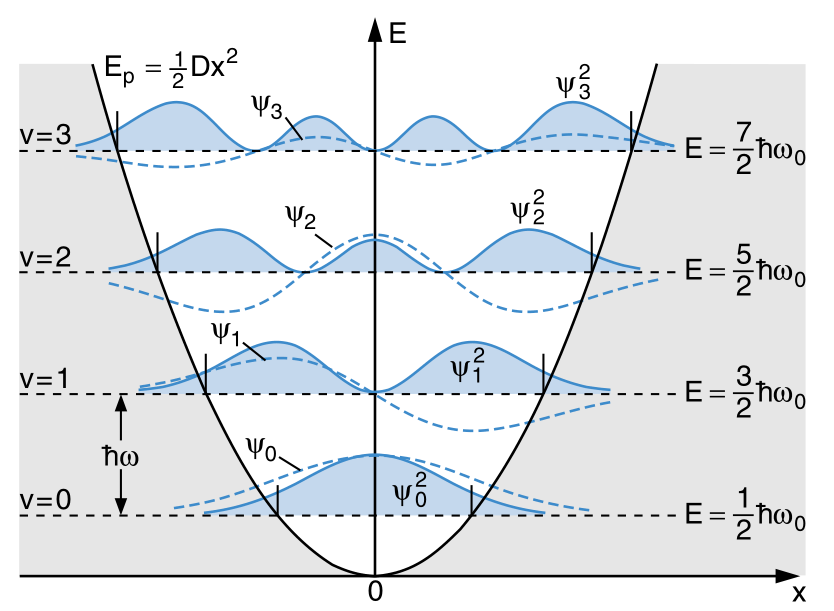
\includegraphics[width=15cm]{pics/harmonic1}
\caption{Energy levels of the harmonic oscillator with its 
    related wavefunctions\cite{Demtroeder1}.}
\label{fig:harmonic1}
\end{figure}
This potential is of outstanding importance for our experiment,
since the real potential will be aproximated in a region near
the minimum with a harmonic potential. 
To a few problems we can find the analytical solution
to the schrödingerequation, but to most
of the problems we need to approximate the solution with regards to an analyical
solution which is given. In the following sections we will introduce
the time-independent Perturbationtheory and give an example with the 
anharmonic oscillator how such an approximation can take place.
\subsubsection{Timeindependent Perturbationtheory}
We are following~\cite{fliessbach2008quantenmechanik}.
Lets assume we know the Eigenvalues and -functions of a specific
Hamiltonoperator $\hat{H_0}$ of the
unperturbed system (we further assume the eigenspaces to be
seperable, so we have no degeneracy. The case of degeneracy
can be done analogously) 
, numbered with $n\in \mathbb{N}$:

\begin{equation}
\hat{H_0} |n\rangle = \epsilon_n |n\rangle 
\end{equation}
and now we search for the solution of the perturbated Hamiltonian:
\begin{equation}
    \hat{H}|\psi \rangle = E|\psi \rangle 
\end{equation}
by means of the initial Hamiltonian:
\begin{equation}
    \hat{H} = \hat{H_0} + \lambda \hat{V}
\end{equation}
where we perturbate the original Hamiltonian with the Potential
$\hat{V}$ and give an approximate Soluation as long as Perturbation
is not of the same order of magnitude as $H_0$. 
The next step will be to apply this to the anharmonic 
Oscillator in order to get an estimation about the energyeigenvalues.
At first we have introduced a new parameter $\lambda$, which is the 
strength of the perturbation; for $\lambda = 1$ we have the problem
we want to solve, for $\lambda = 0 $ we arrive at the unperturbed
problem. Now we can expand in this parameter:
\begin{align}
    E_n(\lambda) &= \epsilon_n + \sum_{\nu =1}^{\infty} \lambda^\nu
    E_{n,\nu} \\ 
    |\psi_n(\lambda)\rangle &=
    |n\rangle + \sum_{\nu =1}^{\infty} \lambda^\nu
    |\psi_{n,\nu}(\lambda)\rangle
\end{align}
As result the solutions we are looking for will become:
\begin{align}
    E_n &= \epsilon_n + E_{n,1} + E_{n,2} + \cdots\\ 
    |\psi_n \rangle &= |n\rangle + |\psi_{n,1} \rangle + \cdots 
\end{align}
We assume for now that this series is converging and plug it into
the Schrödingerequation:
\begin{equation}
    (\hat{H_0} + \lambda \hat{V})
   \left( |n\rangle + \sum_{\nu =1}^{\infty} \lambda^\nu
        |\psi_{n,\nu}(\lambda)\rangle \right) =
\epsilon_n + \sum_{\nu =1}^{\infty} \lambda^\nu
    E_{n,\nu}  
    \left( |n\rangle + \sum_{\nu' =1}^{\infty} \lambda^{\nu'}
        |\psi_{n,\nu'}(\lambda)\rangle \right) 
\end{equation}
Now we can impose that the different powers of $\lambda$ have to
match on both sides and receive a set of equations:
\begin{align}
    \hat{H_0} |n\rangle &= \epsilon_n |n\rangle\\
    \hat{H_0} |\psi_{n,1}\rangle + \hat{V}|n\rangle &=
    \epsilon_n |\psi_{n,1}\rangle + E_{n,1}|n\rangle \label{eq:dev1}\\
    \hat{H_0} |\psi_{n,2}\rangle + \hat{V}|\psi_{n,1}\rangle &=
    \epsilon_n |\psi_{n,2}\rangle + E_{n,1}|\psi{n,1}\rangle 
    + E_{n,2}|n\rangle \label{eq:dev2}\
\end{align}
This set of equations yield recursive the Solutions of $E_{n,1}$,
$E_{n,2}$ and so on. Now we expand these single Wavefunctions 
into the new basis of energyeigenfunctions $|m \rangle$ with $m\in 
\mathbb{N}$:
\begin{equation}
    |\psi_{n,1}\rangle = \sum_{m=1}^{\infty} a_{nm} |m \rangle
    \label{eq:psi_expansion}
\end{equation}
We can plug this expansion now into into equation~\eqref{eq:dev1}:
\begin{equation}
    \sum_{m=1}^{\infty} (\epsilon_n - \epsilon_m) a_{nm} |m\rangle
    + E_{n,1} |n\rangle = \hat{V}|n \rangle
\end{equation}
With the Projection onto the dual eigenstate $\langle k|$ we can
use the orthonormality $\langle k | m \rangle = \delta_{m,k}$ 
of the energyeigenfunctions:
\begin{equation}
     (\epsilon_n - \epsilon_k) a_{nk} 
     + E_{n,1}\delta_{n,k}  = \langle k |\hat{V}|n \rangle
\end{equation}
For the case $k = n$ we get:
\begin{equation}
    E_{n,1} = \langle k |\hat{V}|n \rangle
\end{equation}
and for $k\neq m$:
\begin{equation}
    a_{n,k} = \frac{\langle k |\hat{V}|n \rangle}
    {\epsilon_n - \epsilon_k} \label{eq:a_nk}
\end{equation}
Equation~\eqref{eq:a_nk} together with~\eqref{eq:psi_expansion} 
gives us now:
\begin{equation}
    |\psi_{n}\rangle = |n\rangle + \lambda \sum_{m\neq n}^{\infty}
    \frac{\langle m |\hat{V}|n \rangle}{\epsilon_n - \epsilon_m}  
    |m \rangle + \lambda a_{n,n} + \mathcal{O}(\lambda^2)
\end{equation}
Now we can set $a_{n,n}=0$ (see footnote~\footnote{
Again we can use orthonormality:
\begin{equation*}
    1\overset{!}{=} \langle \psi_n|\psi_{n}\rangle 
    = \left | 1 + \lambda a_{nn} \right |^2 + \lambda^2
    \sum_{m\neq n}^{\infty}
    \left | \frac{\langle m |\hat{V}|n \rangle}
        {\epsilon_n - \epsilon_m} \right |^2 = 
    1 + \lambda (a_{n,n} + a^*_{n,n}) + \mathcal{O}(\lambda^2)
\end{equation*}
When $\lambda > 0 $ this results into:
\begin{equation*}
    a_{n,n} + a^*_{n,n} = 0 \Rightarrow \Re  [a_{n,n}] = 0
\end{equation*}
Since the Wavefunctions 
are invariant with respect to a phase $\phi$,
we can set without limitations $a_{nn}$ to zero.} for
further details) and we arrive
at:
\begin{equation}
    |\psi_{n}\rangle = |n\rangle + \lambda \sum_{m\neq n}^{\infty}
    \frac{\langle m |\hat{V}|n \rangle}{\epsilon_n - \epsilon_m}  
    |m \rangle  + \mathcal{O}(\lambda^2)
\end{equation}
For the Energy we can make use of the third equation and go to
the second order:
\begin{equation}
|\psi_{n,2}\rangle  = \sum_{m=1}^{X} b_{n,m} |m \rangle 
\end{equation}
We can plug this analogously into equation~\eqref{eq:dev2} and
arrive at:
\begin{equation}
 \sum_{m}^{\infty} (\epsilon_n - \epsilon_m) b_{nm} |m\rangle +
 \sum_{m}^{\infty} E_{n,1} a_{n,m} |m \rangle + E_{n,2} |n \rangle =
 \sum_{m}^{\infty} a_{n,m} \hat{V} |m \rangle
\end{equation}
Where again we use the orthonormality. For $k=n$ we get:
\begin{equation}
    E_{n,2} = \sum_{m}^{\infty} a_{n,m} \langle n |\hat{V}|m\rangle
= \sum_{m\neq n}^{\infty}\frac{|\langle n | \hat{V} | m \rangle |^2}
    {\epsilon_n - \epsilon_m}
\end{equation}
For $k\neq n$ we would arrive at the explicit formula for $b_{n,m}$
but this is not necessary for the further computations.
As final result we therefore get:
\begin{align}
    E_n &\approx \epsilon_n + \langle n|\hat{V} | n \rangle +
\sum_{m\neq n}^{\infty}\frac{|\langle n | \hat{V} | m \rangle |^2}
    {\epsilon_n - \epsilon_m} \\
    |\psi_n \rangle &\approx 
    |n\rangle + \sum_{m\neq n}^{\infty}
    \frac{\langle m |\hat{V}|n \rangle}{\epsilon_n - \epsilon_m}  
    |m \rangle 
\end{align}
\subsection{The anharmonic oscillator}
Lets assume we have solved the harmonic oscillator with 
\begin{align}
    \hat{H_0} &= \frac{\hat{p}^2}{2m} 
    + \frac{1}{2} m \omega_0^2\hat{x}^2 \\
    \hat{H_0}|n \rangle &= \epsilon_n |n \rangle \\
    \epsilon_n &= \hbar \omega_0 \left (n+ \frac{1}{2} \right)
\end{align}
Now perturbe this system with a kubic potential potential:
\begin{equation}
\hat{V} =\lambda \hat{x}^3
\end{equation}
Hence we can use the perturbation theory in linear order.
Since the parity of $\hat{V}$ is odd, the expectation value has 
to be zero:
\begin{equation}
    E_{n,1} = \lambda \langle n | \hat{x}^3 | n \rangle = 0 
\end{equation}
The wavefunctions have to be corrected as follows:
\begin{equation}
    |\psi_{n,1} \rangle = \sum_{m\neq n}^{\infty}
    \frac{\langle m |\hat{V}|n \rangle}{\epsilon_n - \epsilon_m}  
    |m \rangle 
    = \frac{\lambda}{\hbar \omega}
    |\psi_{n,1} \rangle = \sum_{m\neq n}^{\infty}
    \frac{\langle m |\hat{x}^3|n \rangle}{\epsilon_n - \epsilon_m}  
    |m \rangle 
\end{equation}
Now we have to calculate the matrix elements. Therefore we
introduce the creation- and annihilationoperator 
which are defined by $\hat{x}$:
\begin{equation}
    \hat{x} = \sqrt{\frac{\hbar}{2m\omega}}(\hat{a}^\dagger +
        \hat{a})
\end{equation} 
Now we can calculate iteratively the matrixelements
\footnote{
    Here we make use how $\hat{a}$ and $\hat{a}^\dagger$ act 
    on the eigenfunctions $|n\rangle$:
\begin{align*}
    \hat{x}|n'\rangle = \sqrt{\frac{\hbar}{2m\omega}}
    \left ( \sqrt{n' + 1}|n'+1\rangle 
        + \sqrt{n'}|n' - 1 \rangle \right ) 
\end{align*}
Applying once more:
\begin{align*}
\hat{x}^2|n'\rangle = \frac{\hbar}{2m\omega}
\left ( \sqrt{(n' + 1)(n' + 2)}|n'+2\rangle 
            + (2n' + 1) |n' \rangle
            + \sqrt{(n'(n'-1)}|n' - 2 \rangle \right ) 
\end{align*}
And applying for the third time:
\begin{align*}
    \hat{x}^3|n'\rangle &= \sqrt[3]{\left (\frac{\hbar}{2m\omega}\right )^2}
( \sqrt{(n' + 1)(n' + 2)(n'+3)}|n'+3\rangle 
    + 3 \sqrt{(n'+1)^3}|n' +1 \rangle  \\
 &+ 3 \sqrt{(n')^3}|n' -1 \rangle   
            + \sqrt{(n'(n'-1)(n'-2)}|n' - 3 \rangle  ) 
\end{align*}
Now this yields the matrixelements which we need:
\begin{align}
    \langle n | \hat{x}^3 | n' \rangle &=  
    \sqrt{\left (\frac{\hbar}{2m\omega}\right)^3}
( \sqrt{(n' + 1)(n' + 2)(n'+3)}\delta_{n,n'+3} 
    + 3 \sqrt{(n'+1)^3}\delta_{n,n'-1}  \\
    &+ 3 \sqrt{(n')^3}\delta_{n,n'-1}   
    + \sqrt{(n'(n'-1)(n'-2)}\delta_{n,n'-3}  ) 
\end{align}

}. After applying the justified indices, since only $n'=n\pm 1$ and
$m = n \pm 3 $ are not zero, we arrive at:
\begin{equation}
\begin{aligned}
    |\psi_{n,1} \rangle &= \frac{\lambda}{\hbar \omega}
    \sqrt{\left(\frac{\hbar}{2m\omega}\right)^3}
    ( -\frac{1}{3}\sqrt{(n + 1)(n + 2)(n+3)}|n+3\rangle 
    - 3 \sqrt{(n+1)^3}|n +1 \rangle  \\
 &+ 3 \sqrt{(n)^3}|n -1 \rangle  
    +\frac{1}{3} \sqrt{(n(n-1)(n-2)}|n - 3 \rangle  ) 
\end{aligned}
\end{equation}
We can also calculate the energy corrections:
\begin{equation}
    E_{n,2} = \langle n | \hat{V} | \psi_{n,1} \rangle 
    = \lambda \langle n | \hat{x}^3 | \psi_{n,1} \rangle 
\end{equation}
Which yields:
\begin{equation}
\begin{aligned}
    E_{n,2} &= \frac{\hbar^2 \lambda^2}{2 m^3 \omega ^4}
    \left[-\frac{1}{3}(n+1)(n+2)(n+3)
        -9(n+1)^3 + 9n^3 + \frac{1}{3}n(n-1)(n-2)
        \right ] \\
    &= -\frac{\hbar^2 \lambda^2}{2 m^3 \omega ^4}
    \left[ 30n^2+ 30n + 11 \right ]\\
    &= -\frac{30 \hbar^2 \lambda^2}{2 m^3 \omega ^4}
    \left[\left(n + \frac{1}{2} \right)^2 + \frac{11}{30} \right ]\\
\end{aligned}
\end{equation}
If we had a look at the closed form for all orders, we would
notice the possibility to expand the Energy Difference in terms
of powers of the original Energy $(n+\frac{1}{2})$ which we will
state here without proof:
\begin{equation}
    E_n = \hbar \omega_{0,0} \left(n + \frac{1}{2} \right) 
    - \hbar \omega_{0,1} \left(n + \frac{1}{2} \right)^2  
    + \hbar \omega_{0,2} \left(n + \frac{1}{2} \right)^3  
    + \cdots
\end{equation}
We did not include the small derivation independent of $n$,
since we will look only at energydifferences. Notice that
the final result is only valid for a small, odd Perturbation. 
\subsubsection{Energylevels and Wavefunctions
    of two-atomic molecules}

First we will write down the full Equations of the two-atomic
molecule and investigate after which parts we can further
simplify (This whole derivation will follow \cite{staatsexamen}):
\begin{equation}
        \hat{H}\psi = E\psi 
\end{equation}
Where we can expand the Hamiltonian in the position-space,
where we already split into the electrons ($i$) and the 
two nucleons $A$ and $B$:
\begin{equation}
    \hat{H} = \frac{-\hbar^2}{2} 
        \underbrace{\left(
        \sum_{i}{\frac{\nabla_i^2}{m_e}}
        +\frac{\nabla_A^2}{M_A} +\frac{\nabla_B^2}{M_B}
\right)}_{
\substack{\text{kinetic energy}\\\text{of electrons and nucleons}}}
+ \underbrace{\sum_{i>j}{\frac{e^2}{|r_i - r_j|}}
    }_{\substack{\text{potential energy}\\\text{electron-electron}}}
 - \underbrace{\sum_{i}{\frac{Z_A e^2}{|r_i - r_A|}}
 }_{\substack{\text{potential energy}\\\text{electron-nucleon $A$}}}
 - \underbrace{\sum_{i}{\frac{Z_B e^2}{|r_i - r_B|}}
 }_{\substack{\text{potential energy}\\\text{electron-nucleon $B$}}}
 +  \underbrace{\frac{Z_A Z_B e^2}{|r_A - r_B|}
 }_{\substack{\text{potential energy}\\\text{nucleon $A$ - nucleon $B$}}}
\end{equation}
Now we split the electronsolutions and the nucleonsolutions such
that the solutions of the electrons change only little when the
distance of the nucleons change, which is known as the
\textsc{BORN-OPPENHEIMER}-Approximation \cite{staatsexamen}:
\begin{align}
    \psi &= \psi_E ( \cdots r_i \cdots) \psi_N(r_A, r_B) \\
    \hat{ H}_E\psi_E &= \left(- \sum_{i}{\frac{\hbar^2\nabla_i^2}{2m_e}}
    + \sum_{i>j}{\frac{e^2}{|r_i - r_j|}}
    - \sum_{i}\frac{Z_A e^2}{|r_i - r_A|}
    - \sum_{i}\frac{Z_B e^2}{|r_i - r_B|}
    + 
    \right ) \psi_E = 
 E_E \psi_E \\
 \hat{H}_N\psi_N &= \left (
 -\frac{\hbar^2\nabla_A^2}{2M_A} -\frac{\hbar^2\nabla_B^2}{2M_B}
    - \sum_{i}\frac{Z_A e^2}{|r_i - r_A|}
    - \sum_{i}\frac{Z_B e^2}{|r_i - r_B|}
 + \frac{Z_A Z_B e^2}{|r_A - r_B|}
 \right ) \psi_N
=  E_N \psi_N 
\end{align}
Where we fixed the positions for the Hamiltonian
of the electrons such that they are not included in the
wavefunction. The interaction between electrons and the nucleons
will not be neglected since the Wavefunctions $\psi_E$ are still
dependend of the distance between the nucleons $r$. 
\par
The obvious problem arises when trying to solve these equations,
since it is not possible without great difficulties. 
The next step is to build up trialsolutions of $\psi_E$, 
consisting of solutions when there is only one electron and a
nucleon. These solutions are called one-electron orbital wave
and will be abbreviated
with \textit{MO} (\textit{Molecule orbital}) and the trialsolutions
will be built up upon linear combinations of those
(\textit{Linear combinations of atomic orbitals} method,
\textit{LCAO}). This method was first introduced 1929 by 
Sir John Lennard-Jones and has to be used with caution, since
it is only in certain limits applicable. The parameters which
appear in these combinations can be constrained by 
expectationvalues measured in experiments.
Now we will turn our attention to the movement of nucleons.
Since in our case we only have two of them, we can perform 
a coordinatetransform to the normal coordinates with a fictional
nucleon with mass
\begin{equation}
    \mu = \frac{M_A M_B}{M_A + M_B}
\end{equation}
so that our new Schrödingerequation with the wavefunction of the
fictional nucleon will look like:
\begin{equation}
    \nabla^2 \psi_N + \frac{2\mu}{\hbar^2} 
    \left[ E - V(r) \right] = 0 
\end{equation}
The Laplaceoperator written in spherical coordinates will yield
the spherical harmonics as eigenfunctions, so we can use a 
seperational ansatz for our wavefunction:
\begin{equation}
    \psi_N(r,\theta,\rho) = \frac{1}{r} S(r)Y(\theta,\rho)
\end{equation}
with the corresponding
differentialoperator, where $J\in \mathbb{N}_0$
corresponds to the Quantumnumber of the total angular momentum:
\begin{equation}
    \frac{\partial}{\sin\theta \partial \theta}\left (\sin\theta
    \frac{\partial Y}{\partial \theta}\right ) +
\frac{1}{\sin^2\theta} \frac{\partial^2 Y}{ \partial\rho^2}
 + J(J+1)Y = 0
\end{equation}
Thus we can split the rest of the wavefunction into the 
radial component of the Operator:

\begin{equation}
    \frac{d^2 S}{dr^2} + \frac{2\mu}{\hbar^2}
\left ( E - V(r) - \frac{J(J+1)\hbar^2}{2\mu r^2} \right ) S =0 
\end{equation}

If there is no further degeneracy (for instance due to not
considered interactions like spin) we can in theory write
down the Energyeigenvalues in terms of the two Quantumnumbers
$nu$ and $J$:
\begin{equation}
    E = E_{\nu,J}
\end{equation}
Practically this is not possible, so we look at two extrem cases.
\paragraph{The rigid Rotator} is based on the approximation to
fix the range of the two nuclei ($r =$const.) and so we only
look at $V(r)=0$ and $\frac{S(r)}{r} = 1$. We immedeatly get
the solution (since the sphericalharmonics already resolved
the eigenvalues):
\begin{equation}
    E = \frac{J(J+1)\hbar^2}{2\mu r^2}
\end{equation}
\paragraph{The rotationless Oscillator} just neglects the terms
arising from rotation, which is, looking at the lengthscale of
the former calculated eigenvalues, not inopportune.
The Operator then becomes:
\begin{equation}
    \frac{d^2 S}{dr^2} + \frac{2\mu}{\hbar^2}
    \left ( E - V(r) ) = 0 \right )
\end{equation}
The Eigenfunctions and -values are now very dependent on the 
potential energy $V(r)$ which is until now not a known 
potential, because it includes the repulsion due to the
pauliprinciple of the electronorbits as well as the attraction
of the charges. Furthermore the physical nature of dissociation
of the two nucleons also has to be encoded into it.
It is not possible to solve the potential analytically, but 
we will start to write down the properties already known:
\begin{itemize}
        \item Pauliprinciple:
            $\lim\limits_{r \rightarrow 0}{V(r)} = \infty $
        \item Dissociated nucleons:
$\lim\limits_{r \rightarrow \infty}{V(r)} = const. $
\item Before the Dissociation: Attraction of the nucleons with
    the maximal attraction at $r_e$ and the Dissociationenergy
    $D_e$ defined by 
    $ \lim\limits_{r \rightarrow \infty}{V(r)} - V(r_e)=: D_e$ 
\end{itemize}
The idea is now to capture this properties into the coefficients
of the taylored Potential and by doing so resolving the principle
physical behavior:
\begin{equation}
    V(r) = V(r_e) 
   + \frac{\partial V(r)}{\partial r}|_{r=r_e}(r - r_e)
   + \frac{\partial^2 V(r)}{2!\partial r^2}|_{r=r_e}(r - r_e)^2
   + \frac{\partial^3 V(r)}{3!\partial r^3}|_{r=r_e}(r - r_e)^3
   + \cdots
\end{equation}
As first approximation for energies near the minimum $r=r_e$ we
can finally use the harmonic potential. The constant term
$V(r_e)$ can be dropped since we are only interested in 
potential differences.
\begin{equation}
    V_{harm}(r) =
    \frac{\partial^2 V(r)}{2\partial r^2}|_{r=r_e}(r - r_e)^2
    =: \frac{k_e}{2}(r-r_e)^2
\end{equation}
Following this approach we can use the energyeigenvalues of the
harmonic oscillator in order to approximate
the vibrational states $\nu$:
\begin{equation}
    E_\nu =\sqrt{\frac{k_e}{\mu}}\hbar \left (\nu
        + \frac{1}{2}\right )
\end{equation}
In order to chose a more convenient unit we transform this
equation into $cm^{-1}$:
\begin{equation}
    G_{harm}(\nu) = \frac{E}{hc} = \omega_0 (\nu + \frac{1}{2})
    \quad \text{with the frequency} \quad
    \omega_0 = \frac{1}{2\pi c} \sqrt{\frac{k_e}{\mu}}
\end{equation}
The wider we leave the regime around $r_e$, speaking about 
higher vibrational states, the worse approximation with a harmonic
oscillator becomes. Qualitatively this is the case when energies
come nearer to the dissociation energy. An adhoc solution is 
to treat this with the already mentioned perturbationtheory in such
a way that we use the condition
\begin{equation}
    \frac{\partial V(r)}{\partial r}|_{r=r_e}        \gg
    \frac{\partial^2 V(r)}{2!\partial r^2}|_{r=r_e}  \gg
    \frac{\partial^3 V(r)}{3!\partial r^3}|_{r=r_e}  
    \cdots
\end{equation}
and can therefore justify the Ansatz:
\begin{equation}
    G(\nu) = \omega_e (\nu + \frac{1}{2} ) 
    - \omega_e x_e (\nu + \frac{1}{2} ) ^2 
    + \omega_e y_e (\nu + \frac{1}{2} ) ^3 
    - \omega_e z_e (\nu + \frac{1}{2} ) ^4 
    + \cdots 
\end{equation}
Since in the experiment it is clearly impossible to seperate
the incoming higher frequencies, we will treat $\omega_e x_e$ as 
one variable, similarily to the others, where they also connected
on lengthscales by
\begin{equation}
    \omega_e \gg \omega_ex_e \gg \omega_e y_e \cdots 
\end{equation}
As before we can shift the equations to make them more convenient,
in this case to scale them to the zeroenergy
\begin{equation}
    G \mapsto G_0 := \left [G-G(0) \right ] 
        \quad \text{which is given by}
    \quad G(0)=\frac{1}{2}\omega_e - \frac{1}{4}\omega_e x_e 
    + \frac{1}{8} \omega_e y_e + \cdots 
\end{equation}
So we get for the shifted term:
\begin{equation}
    G_0(\nu) = 
\end{equation}
\clearpage



\section{Setup and procedure}
First we give an overview of the program which constitutes the experiment. In another subsection, 
we give a describtion of the setup used. 
\subsection{Procedure}
The procedure of measurements consists of the following six points:
\begin{enumerate}
    \item 
        \textbf{Assessing the detectors and probe at hand with the oscilloscope:}
        We measure the signals of the preamplifier (PA) as wel as uni- and bipolar outputs of 
        main amplifier (MA) at the oscilloscope. With this signal, we calculate the ascending time 
        of the signal.
    \item 
        \label{it:task2}
        \textbf{recording the energy spectrum of $^{57}$Co and $^{241}$Am:}
        The multichannel analyzer (MA) we measure the energy spectrum of both probes 
        for ca. 10 minutes. With the $^{57}$Co sample, we test the sensibility of each detector
        and the optimal positioning of the sample (which is not symmetric). After assigning the 
        channel-energy relationship based on the knowledge of some peaks, we interprete the other visible peaks.
    \item
        \textbf{setting the energy windows:}
        In this step, we restrict the events passed by the single channel analyzer (SCA) to those 
        of the 14.4 keV and 122 keV photons, respectively.
    \item
        \textbf{measuring the delayed coincidences:}
        Using the Time-to-Amplitude converter (TAC), we record the delays between 14.4 keV and 122 keV 
        events. Since the 14.4 keV photon is only emitted in 10 \% of the cases, we use this signal to start the 
        TAC, and stop with the delayed 122 keV photon, expecting to drastically reduce the dead time of the 
        measurement.
    \item
        \textbf{measuring the background (random coincidences):}
        Taking out the delay of the 122 keV signal and further introducing a delay on the 14.4 keV signal, 
        we measure the background. 
    \item
        \textbf{time calibration of Time to Amplitude converter (TAC):}
        In order to correlate measured channel and the respective time delay, we measure the channel 
        assigned by TAC and MCA corresponding to a known delay and perform a fit a linear function between 
        the two quantities. This correspondance will be used in the anaylsis of the delayed coincidences. 
\end{enumerate}


\subsection{Experimental setup}
The setup of the experiment consists of a fixed part with probe and a detector at each side 
as well as a part with the electronics. The devices are adapted to each part, as described below. 

A photo of the two detectors and the probe is shown in figure \ref{fig:position_1}. The given setup also 
defines position 1, later referred to as "Pos1" (see table \ref{tab:config2}). Position 2 ("Pos2") corresponds 
to the probe rotated by $180^\circ$. From its geometry, one can already suspect that the number of photons 
that can be measured from either direction is not equal. A similar condition is true for the detectors:
Already on the first glance, it is clear that the two are not of the same model. In fact, the left detector 
is an older model and suspected to be less sensitive. A more quantitative statement will be made in the 
of the second part of the experiment (see \ref{it:task2}).

\begin{figure}[H]
    \centering
    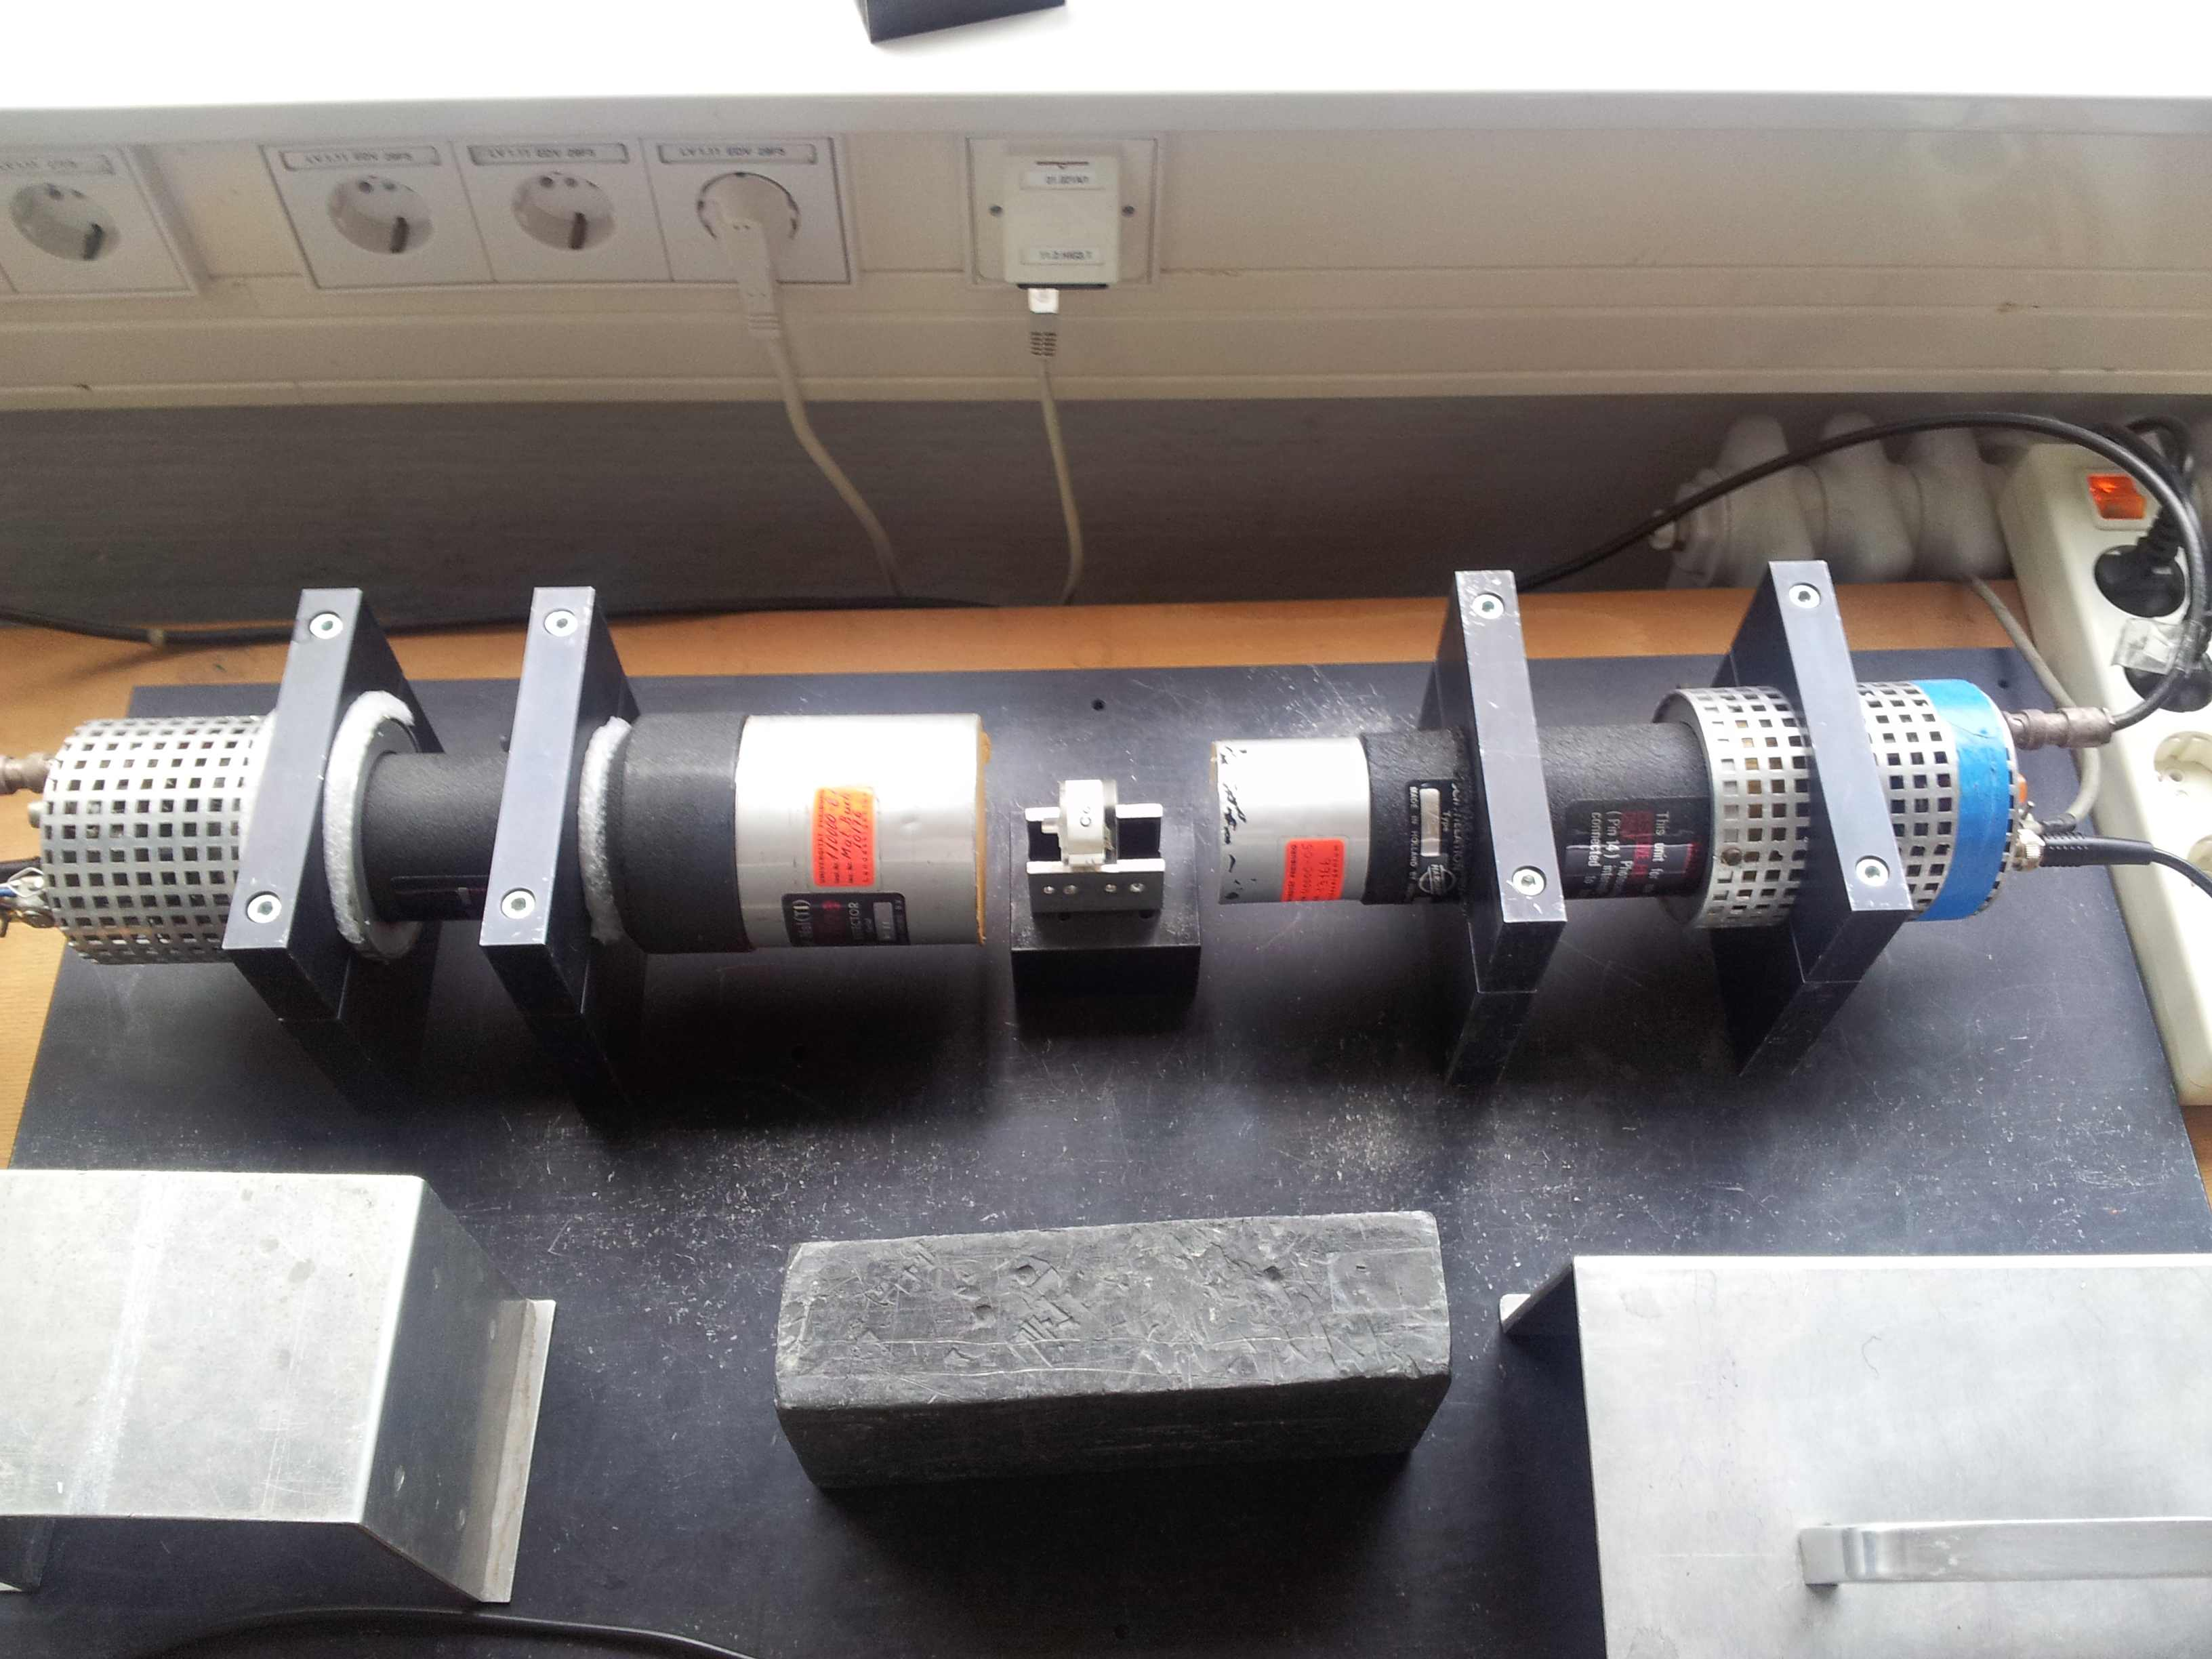
\includegraphics[width=0.8\linewidth]{figures/position_1.jpg}
    \caption{
        Photo of the $57$^Co probe and the two detectors with the setup used in the 
        experiment. The orientation of the probe is the one used for the measurement of 
        the delayed coincidences, with the larger opening facing the right detector. 
        During the measurements, the probe is isolated by the 
        }
    \label{fig:position_1}
\end{figure}




\section{Evaluation}
\subsection{Band Gap}
The raw data is plotted in figure \ref{fig:band_gap_raw_Ge} for 
germanium and \ref{fig:band_gap_raw_Si} for silicon. 
We set the $U-I$-converter to $15.03 \pm 0.03\,$mA for Ge 
and $0.75 \pm 0.01\,$mA for Si. The aperture was opened to 
$-10.0$--$+10.0\,$mm for both samples. Further settings 
not relevant for the evaluation, such as the settings of the gains, 
can be looked up in the 
handwritten records of the experiment in the appendix, 
\ref{sec:records_band_gap}. 
\begin{figure}
    \centering
    \begin{subfigure}[b]{\pltw}
        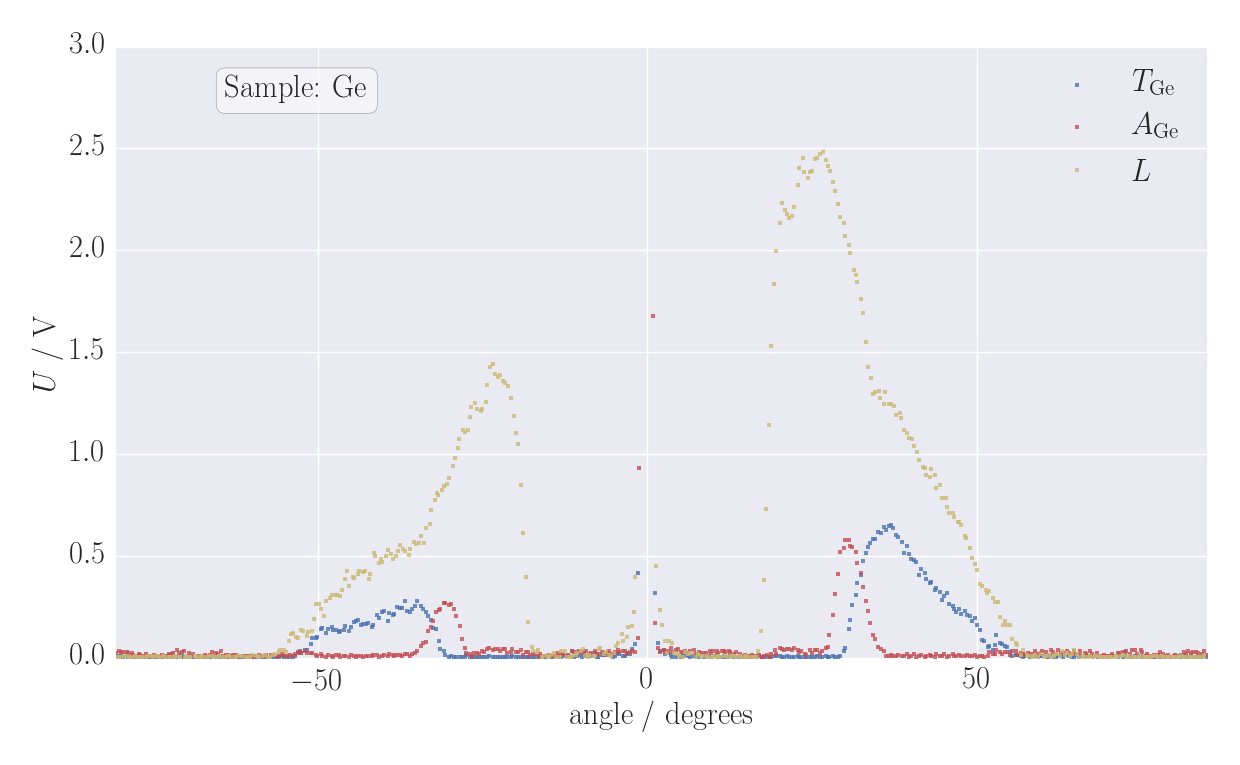
\includegraphics[width=1.0\linewidth]{figures/band_gap_raw_Ge}
        \caption{}
        \label{fig:band_gap_raw_Ge}
    \end{subfigure}
    \begin{subfigure}[b]{\pltw}
        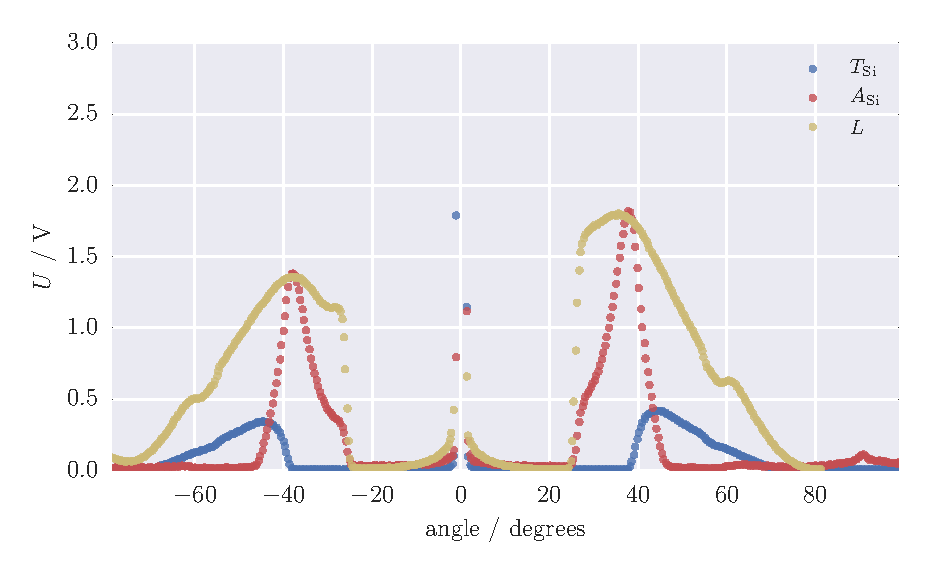
\includegraphics[width=1.0\linewidth]{figures/band_gap_raw_Si}
        \caption{}
        \label{fig:band_gap_raw_Si}
    \end{subfigure}
    \caption{
        The signals measured with Ge (\ref{fig:band_gap_raw_Ge}) 
        and Si (\ref{fig:band_gap_raw_Si}) as samples with corresponding 
        grating and filter. $T$ and $A$ indicate 
        the transmission and absorption, measured by the currents through 
        the pyrodetector and the semiconductor, respectively. 
        $L$ is the intensity of the lamp with installed filter, measured 
        without the semiconductor. The asymmetry might be due to 
        irregularities on the grating or within the beam path. 
        }
    \label{fig:band_gap}
\end{figure}

The evaluation for both samples is done 
absolutely analogously. We thus explain the steps for the example 
of Ge plotting all necessary steps, while the plots for 
Si are added to the appendix, \ref{sec:appendix_band_gap_plots}.
In order to apply the formulas \eqref{eq:t_real} and \eqref{eq:a_real}
for the real transmission and absorption, we had to interpolate the data, 
because the angles measured for all three quantities involved did 
non agree. From each data set, e.~g. angles $\phi$ and measured transmission $T$ 
and absorption $A$ with the Ge sample installed, we created a traverse function 
interpolating $T$ and $A$ on a predefined grid. 
Calculating $T$ at angle $\phi$ was done in the following manner:
Let $(\phi_1, T_1)$ and 
$(\phi_2, T_2)$ be the pairs of data with $\phi_1$ and $\phi_2$ the 
next angles on the left and right of $\phi$, respectively. 
Then, 
\begin{equation}
    T = \frac{1}{(\phi_2 - \phi_1)} 
        \left(T_1\left(\phi - \phi_1\right) + T_2\left(\phi_2 - \phi\right)\right)
\end{equation}

The result of this procedure can be seen in figure~\ref{fig:band_gap_detail_Ge_left}, 
showing a detail of the entire spectrum on the left side ($\phi < 0^\circ$). 
This figure will not be shown for the other side or the Si sample, as 
it has only exemplary character. 
Seeking the intersect of the straight lines interpolated at the transition from 
absorption to transmission is done on yet a smaller scale. Here, 
the signals are normalized, setting $T = 1$ and $A = 1$ for the according maxima, 
when the antagonist is close to zero. The fit is then done choosing the 
points which are used manually. The results together with the points chosen for fitting 
are displayed in figure~\ref{fig:band_gap_result_Ge_left}. 
\begin{figure}
    \centering
    \begin{subfigure}[b]{\pltw}
        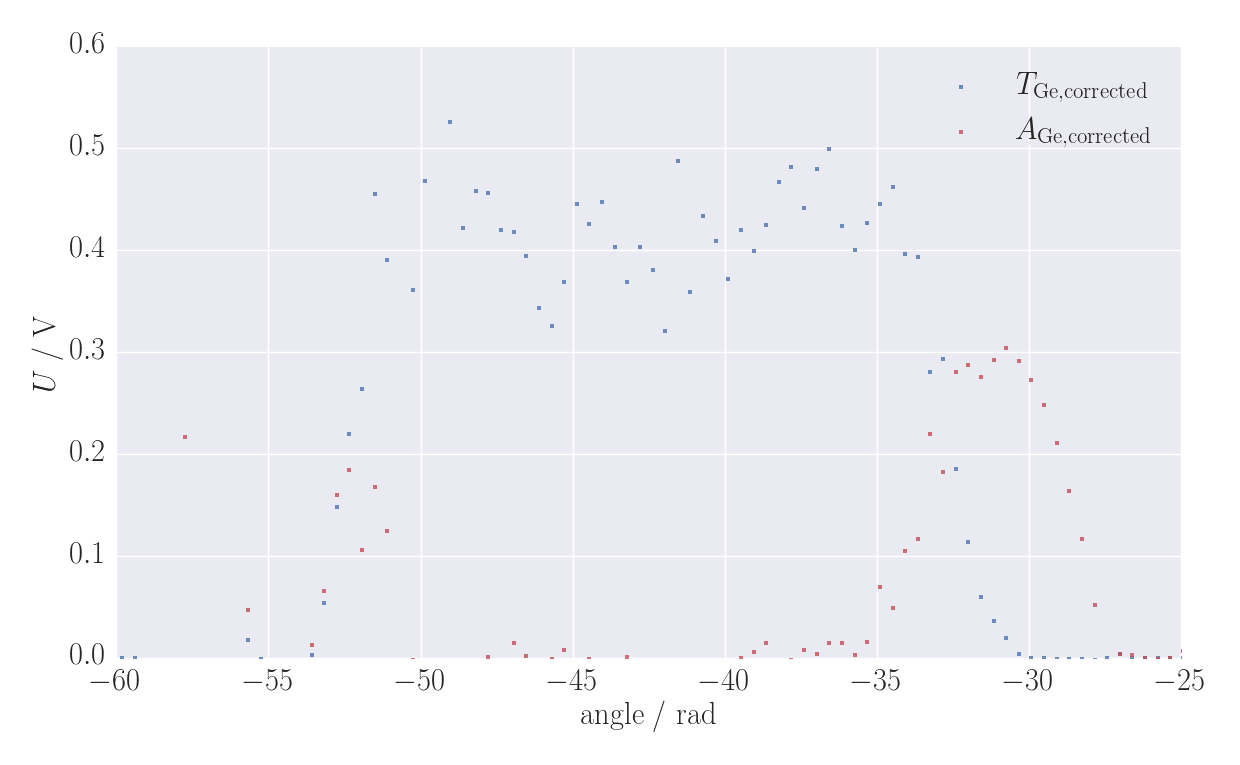
\includegraphics[width=1.0\linewidth]{figures/band_gap_detail_Ge_left}
        \caption{
            Detail of the transmission and absorption, corrected for the 
            background and the spectrum of the lamp. The region we are interested 
            in for further evaluation if the intersect of $T$ and $A$ in
            the right half of the plot. 
            }
        \label{fig:band_gap_detail_Ge_left}
    \end{subfigure}
    \begin{subfigure}[b]{\pltw}
        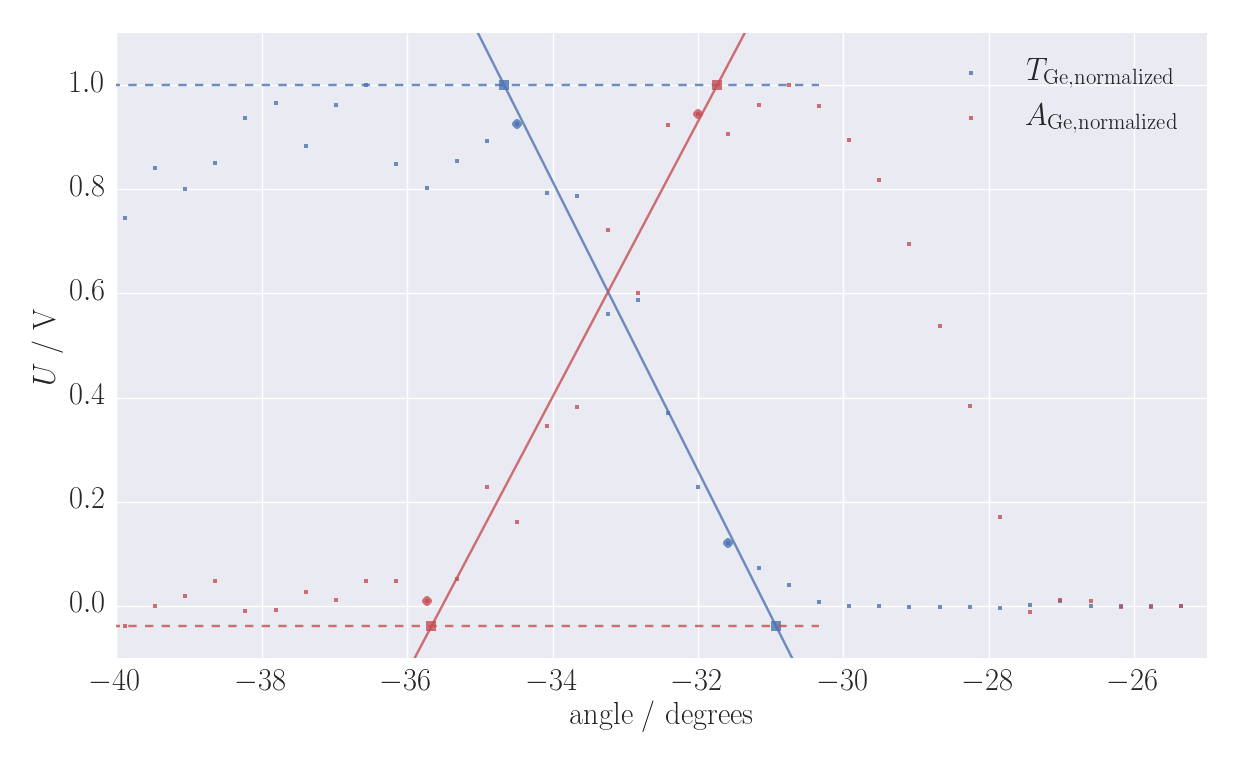
\includegraphics[width=1.0\linewidth]{figures/band_gap_result_Ge_left}
        \caption{
            Result of the procedure fitting straight lines through the points 
            at the transition from transmitting to absorbing characteristic. 
            The larger round dots indicate the upper and lower limit 
            chosen for the interpolation. The dashed line corresponds to 
            the maximum of transmission and minimum of absorption, the 
            squares to the respective intersects with the straight lines.
            In order to maintain clarity, 
            the values for the angles at the intersects are given in the text. 
            The nominal value for the band gap energy is given by the intersect 
            of the two lines. 
            }
        \label{fig:band_gap_result_Ge_left}
    \end{subfigure}
    \caption{
        Plots corresponding to the calculation of $\alpha_g$ which is then be 
        used to calculate the band gap energy $E_g$. 
        }
    \label{fig:band_gap_result_Ge}
\end{figure}
The band gap energy is thus reached for an angle of $\phi_g = 123^\circ$, 
which applying equation~\eqref{eq:E_g} yields:
\begin{equation}
    E_g = 123
\end{equation}
One can observe BLABLABLABLABL

For the right side, the respective plot is shown in the appendix, 
figure~\ref{fig:band_gap_result_Ge_right}, followed by those for the 
silicon (\ref{fig:band_gap_result_Si_left}, \ref{fig:band_gap_result_Si_right}). 
The results are displayed in table \ref{tab:band_gap_results}.

\subsection{The Haynes \& Shockley experiment}
\subsubsection{Measuring at constant $U$}
In this first part, we measured the response in the germanium block to 
the laser pulse at constant voltage $U = (49.6 \pm 0.8)\,$V, 
changing the distance between the point where the laser enters 
and the needle $d$ over a range from 1 to 10 mm. 

Taking the measurements, we had to cope with various difficulties. 
Most notably, the observability of even the signal 
of the laser itself ceased at one point, probably due to the needle 
loosing contact or other technical issues. 
After trying to readjust the setup, we did observe a signal 
again. 
Only doing the evaluation did we notice that this also resulted in 
a large offset in time for all following measurements. 
Thus, the first four measurements have to be ignored. The offset 
remained stable for all but one ('File 7') of the further measurements. 
Furthermore, another set was so badly influenced by noise that 
a gaussian fit has no chance to converge. 
For the remaining data, we apply the following scheme: 
In order to facilitate the convergence of the fitting algorithm, 
we took the according set of smooth data, which is simply the 
average of 128 measurements done by the oscilloscope. 
The resulting parameters are then passed to the algorithm
as initial guesses for a fit on the original data. 
This is shown for an exemplary case in figure \ref{fig:h_s_raw_28}, 
where the measured distance $d$ has been measured to 
$d = 3.7 \pm 0.5\,$mm. 
The parameters obtained by the fit with the original data 
are shown in a box within the plot as well. 
The fitted offset is omitted as it will not be used in any further 
calculation. The errors 
are obtained by the fitting algorithm as the square root of the 
diagonal entries. We did not further add an error on the 
$U$-value, as the scattering should be indication of 
uncertainty enough. For the oscilloscope, only 
a DC vertical accuracy is stated which would 
only apply for the offset. 
In the further calculations, we ignore the 
off-diagonal elements since the desired quantities each depend 
on only one parameter. 
\begin{figure}
    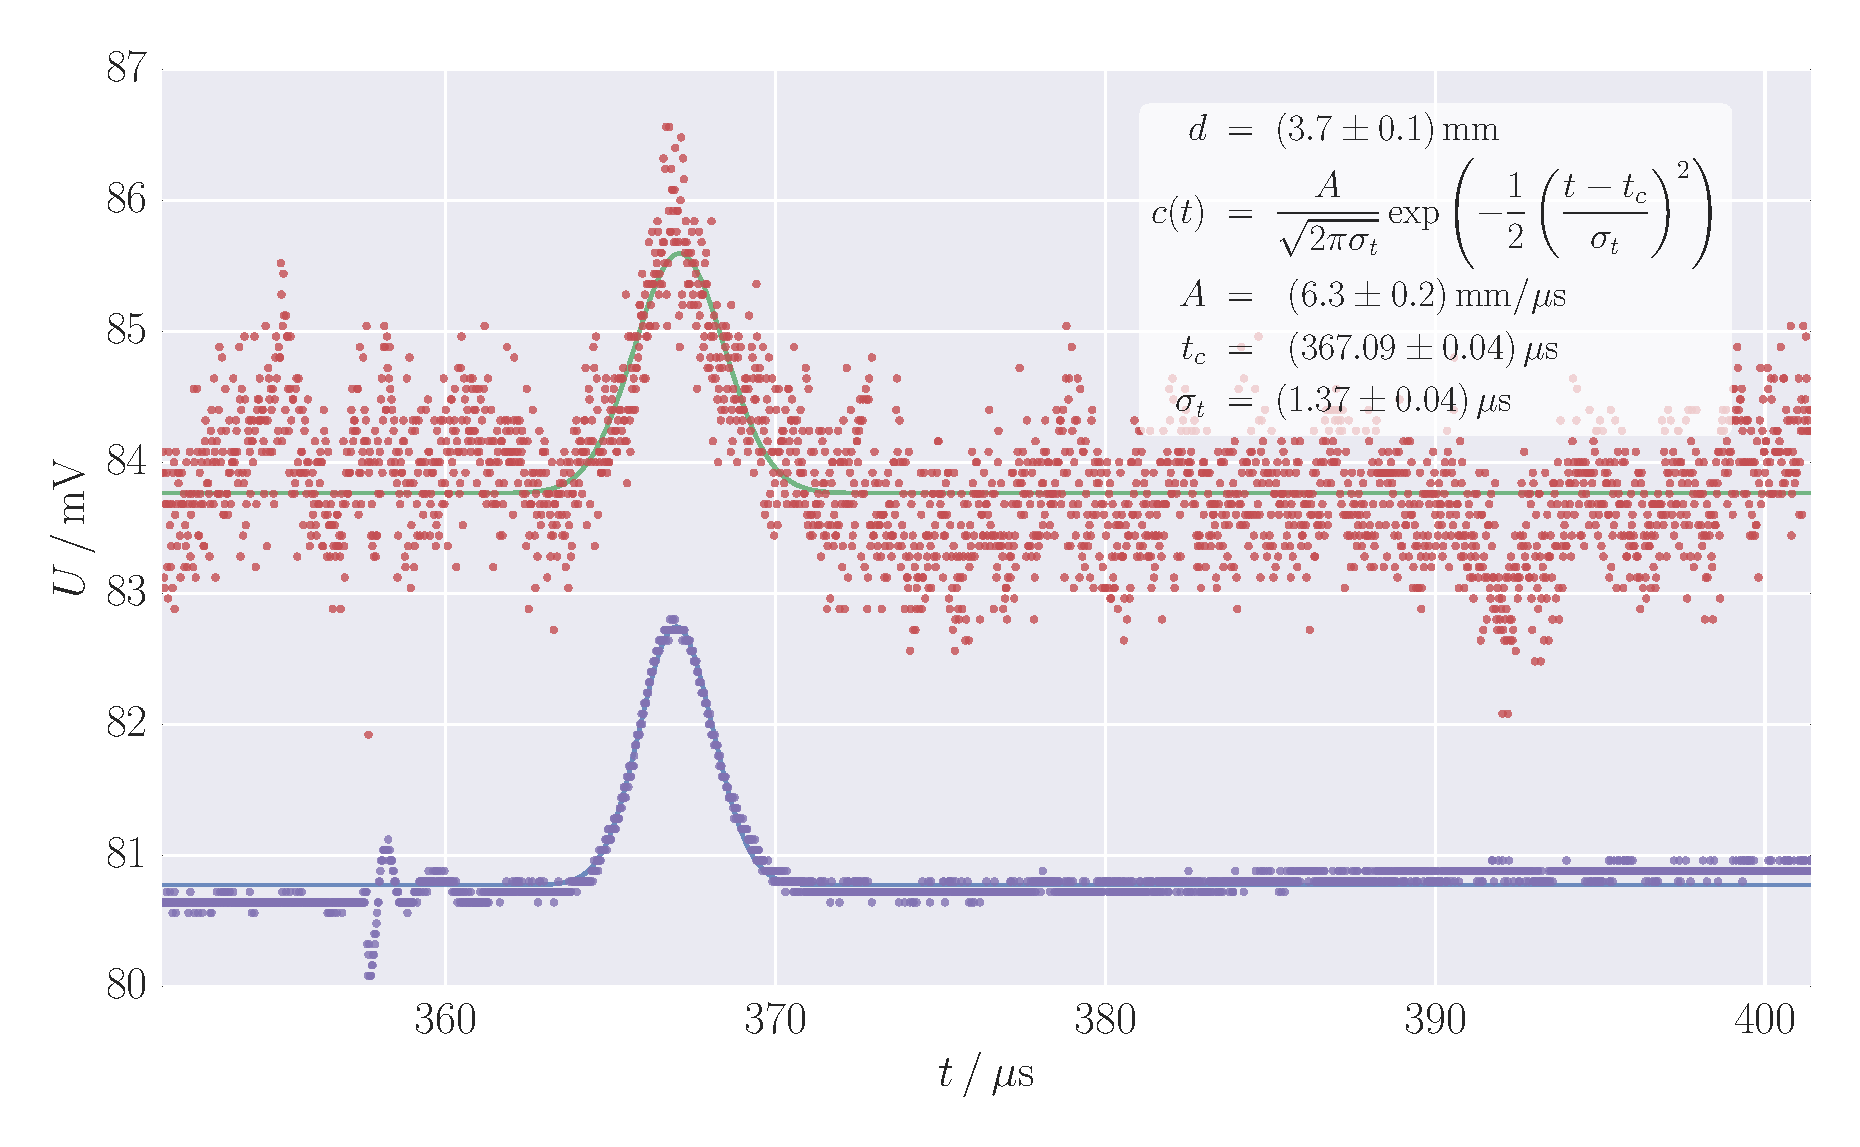
\includegraphics[width=1.0\textwidth]{figures/haynes_shockley_raw_28}
    \caption{
        Raw data and fitted gaussians for $d = 3.7 \pm 0.5\,$cm. 
        The lower, much more scattered data is taken without averaging 
        while the upper corresponds to the average of 128 measurements, where the 
        running average is done by the oscilloscope directly. This smoother data is 
        used to obtain the guesses for the fit on the noisy data, 
        while all further calculations are done with the original, 
        non-averaged data. 
        One can observe the large offset which is of unknown origin appearing 
        after a temporary loss of signal and small adjustments on the setup.
        }
    \label{fig:h_s_raw_28}
\end{figure}

Plots of all used data (original and smooth ones) with the 
fitted functions drawn are shown in the appendix, 
see~\ref{sec:appendix_h_s_plots}.
For all further calculations, the smoothed data is ignored 
and each calculation is done with the non-averaged ones. 
Errors will always be taken to be those of the fits.
An overview of the fitted parameters at corresponding 
distance $d$ is given in table~\ref{tab:h_s_fit_parameters}.
\renewcommand{\arraystretch}{1.5}
\begin{table}[htdp]
    \centering
    \caption{
        Results of fits with gaussians for all used data sets with distance 
        $d$ between laser and needle. The $\chi^2$-tests are quite high due to the 
        noise and tendencies to ascend on the scale of 10 sigma (compare figures, 
        e.~g.smooth data in figure~\ref{fig:h_s_raw_28}).
        }
    	\begin{tabular}{|p{2cm}|p{3cm}|p{3cm}|p{3cm}|p{2cm}|}
		\hline
		\rowcolor{tabcolor}
		$d \, / \, \mathrm{mm}$        & $A \, / \, \mathrm{\frac{mm}{\mu s}})$ & 
 			$t_c \, / \, \mathrm{\mu s}$    & $\sigma_t \, / \, \mathrm{\mu s}$ & 
 			$\chi^2 / n_d$ \\ \hline
		$7.5$ & $3.2 \pm 0.2$ & $377.54 \pm 0.13$ & $1.93 \pm 0.13$ & $10.2$\\ 
		$8.5$ & $3.3 \pm 0.3$ & $378.28 \pm 0.20$ & $1.98 \pm 0.20$ & $3.0$\\ 
		$8.0$ & $2.5 \pm 0.3$ & $377.58 \pm 0.20$ & $1.69 \pm 0.20$ & $2.8$\\ 
		$7.5$ & $2.7 \pm 0.2$ & $376.50 \pm 0.11$ & $1.23 \pm 0.11$ & $2.6$\\ 
		$5.9$ & $3.0 \pm 0.2$ & $372.45 \pm 0.09$ & $1.05 \pm 0.09$ & $3.4$\\ 
		$4.4$ & $4.0 \pm 0.2$ & $368.91 \pm 0.05$ & $1.14 \pm 0.05$ & $9.9$\\ 
		$3.9$ & $3.8 \pm 0.2$ & $367.71 \pm 0.05$ & $1.12 \pm 0.05$ & $12.3$\\ 
		$3.7$ & $6.3 \pm 0.2$ & $367.09 \pm 0.04$ & $1.37 \pm 0.04$ & $12.3$\\ 
		$1.1$ & $12.2 \pm 0.2$ & $362.66 \pm 0.01$ & $0.95 \pm 0.01$ & $12.3$\\ 
		\hline
	\end{tabular}

    \label{tab:h_s_fit_parameters}
\end{table}

The obtained center of the gaussians $t_c$ are plotted over the 
according distances. With a linear fit, we calculate $\mu_n E$. 
The results are shown in figure~\ref{fig:h_s_mu_e_d}. 
With the length $l = (3.0 \pm 0.5)\,$mm for the germanium strip and 
applied voltage $U = (49.6 \pm 0.8)\,$V we calculate an electric field of 
\begin{equation}
    E = \frac{U}{d} = (1.65 \pm 0.04)\, \mathrm{\frac{V}{mm}}\, .
\end{equation}
The electron mobility is then calculated to 
\begin{equation}
    \begin{split}
        \mu_n   &= (0.264 \pm 0.013)\, \mathrm{\frac{mm^2}{V\mu s}} \\
                &= (2640 \pm 130)\, \mathrm{\frac{cm^2}{V\,s}} \,.
    \end{split}
\end{equation}
Although the literature value~\cite{staatsexamen} of 
\begin{equation}
    \mu_{n, \mathrm{lit}} = 3900\, \mathrm{\frac{cm^2}{V\,s}}
\end{equation}
is far off the measured value (by 10 standard deviations --  showing the 
    enormous underestimation of systematical errors applying purely 
    intrinsic estimation and propagation), the calculated value 
does agree in magnitude. It is further expected that the physical 
reality under consideration, namely the electrons moving close to the surface 
of the sample, does change all parameters considerably. 


\begin{figure}
    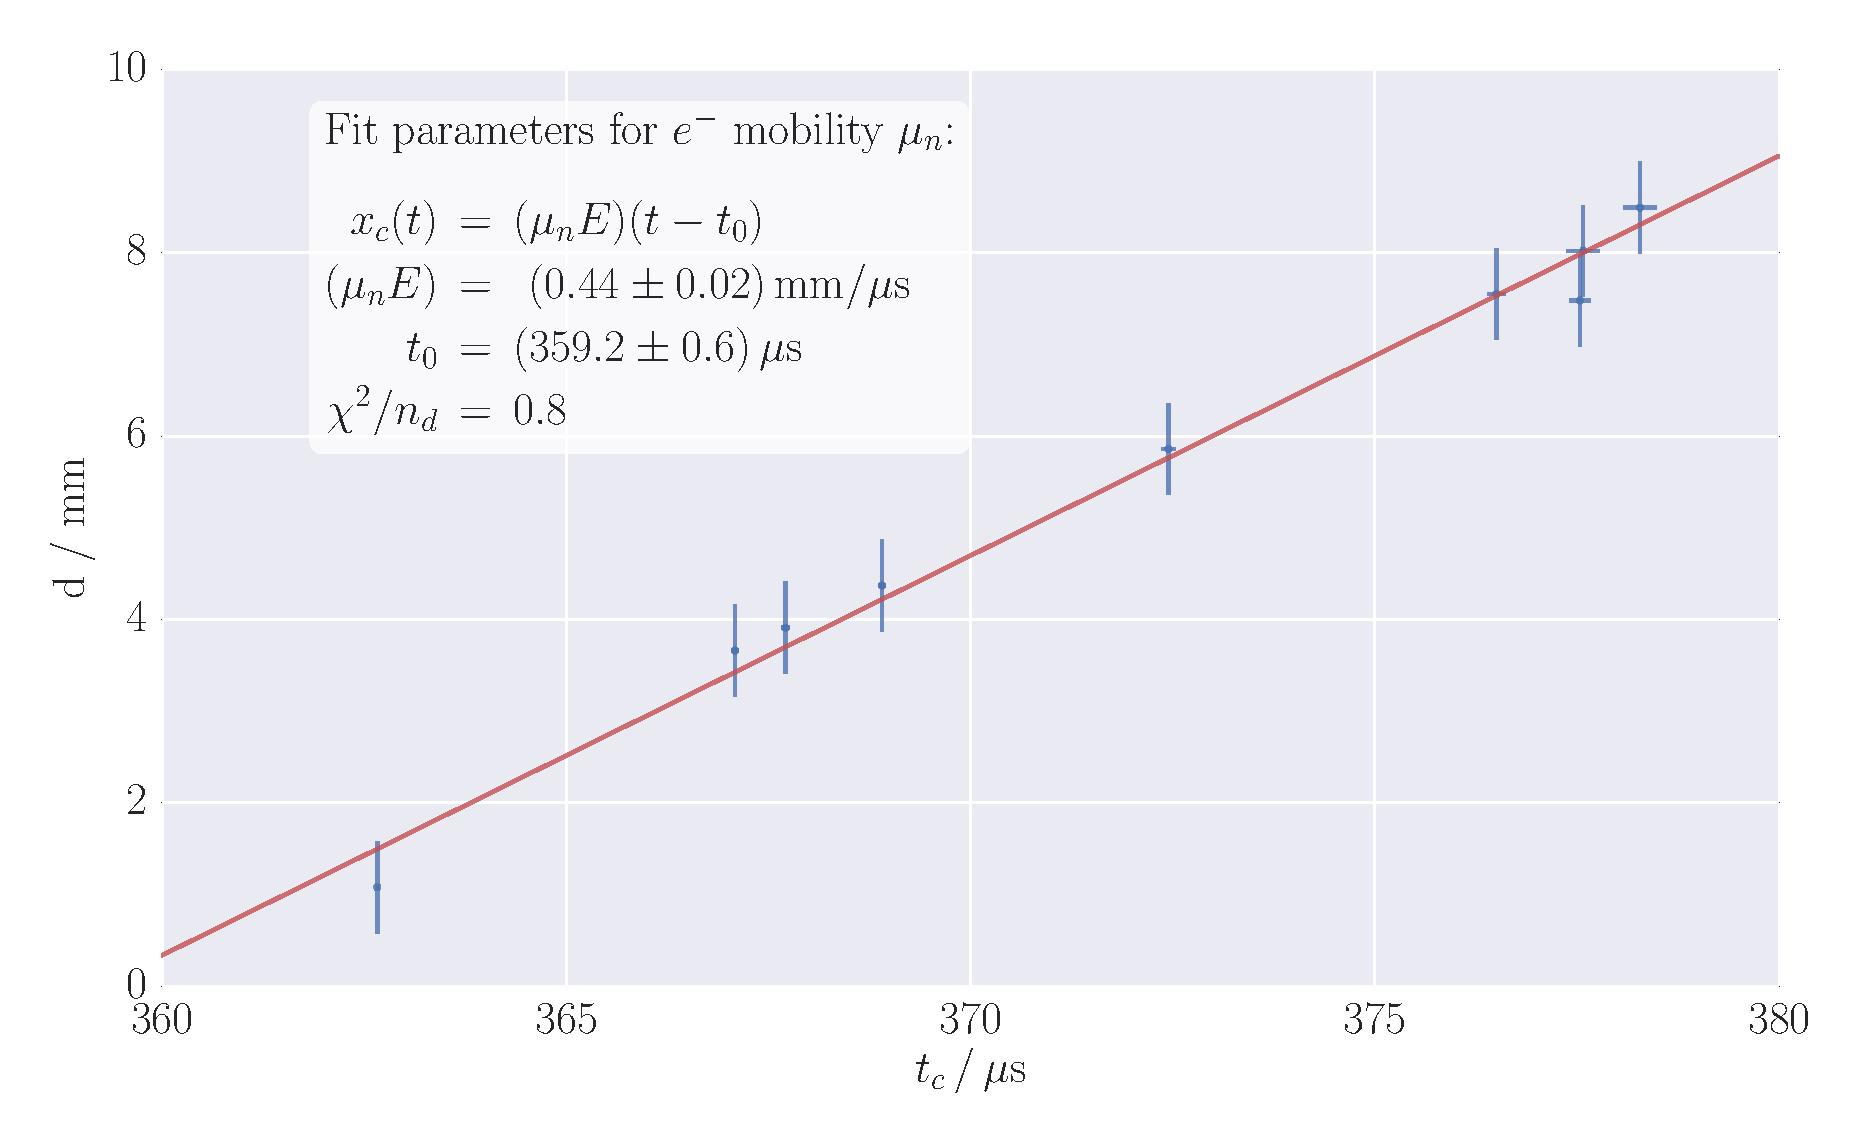
\includegraphics[width=1.0\textwidth]{figures/haynes_shockley_mu_e_d}
    \caption{
        Fitted straight line on centers of gaussians as calculated before. 
        The linear behavior is see quite well, as indicated also by the 
        $\chi^2$-test.
        }
    \label{fig:h_s_mu_e_d}
\end{figure}

With the velocity $v = \mu_n E$ calculated, we can transform 
the temporal sigma to a spatial one as described in the procedure section~%
\ref{sec:transform_x_t}. We can then perform the exponential fit on 
the amplitudes $A(t_c)$ at the maximum, as shown in figure~\ref{fig:h_s_tau_d}.
Here, the fit does not yield such a good result. The errors obtained 
by the gaussian fits seem to underestimate the real uncertainty 
which might be subject to several systematic errors, as will be described later on. 
The life time $\tau_n$ of the electrons is a yielded directly by the fit:
\begin{equation}
    \tau_n = (6.7 \pm 1.0)\, \mathrm{\mu s} \, .
\end{equation}
The literature value $\tau_{n, \mathrm{lit}} = (45 \pm 2)\, \mathrm{\mu s}$%
~\cite{staatsexamen}
is one magnitude above our results. Aside the systematical errors already 
mentioned, the measured value corresponds to a somewhat different 
physical reality: As the laser only enters the first $0.5 \, \mathrm{\mu m}$
of the sample~\cite{staatsexamen}, we expect the lattice defects to have 
a large effect especially on the recombination rate. Theoretically, 
these effects are much harder to calculate -- experimentally, however, 
it turns out that the defects drastically reduce the life time of free electrons. 

\begin{figure}
    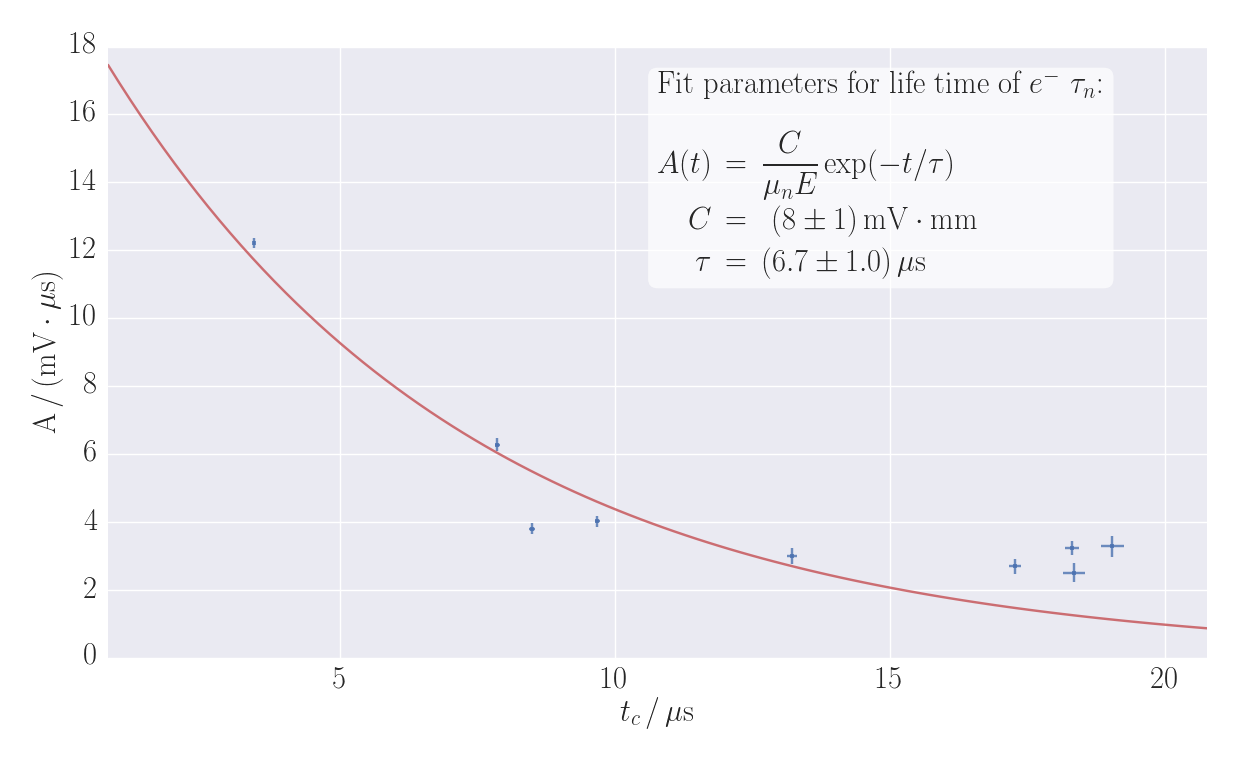
\includegraphics[width=1.0\textwidth]{figures/haynes_shockley_tau_d}
    \caption{
        Exponential fit through the amplitudes obtained by the gaussian fits 
        in order to calculated the electron life time $\tau$. The $\chi^2$-test 
        as well as the graphical impression shows that the errors obtained by the 
        linear regression do not mirror the fluctuations obtained. It could 
        further be the case that systematical errors have a large impact on the 
        data. 
        }
    \label{fig:h_s_tau_d}
\end{figure}

In the ultimate part of evaluating this measurement, the standard deviations in 
time $\sigma_t$ are transferred to those in space $\sigma_x$ as described before. 
The spatial variances $\sigma_x^2$ are then fitted linearly over the time 
traveled by the electrons $t_c$. The result is shown in figure~\ref{fig:h_s_D_d}.
Even more so then in the prior fit the data does not show the expected behavior 
but instead fluctuates widely due to the systematical errors and noise. 
The obtained value of electron diffusion constant 
\begin{equation}
    D_n = (140 \pm 20)\, \mathrm{\frac{cm^2}{s}} 
\end{equation}
can thus be regarded only as an assessor of the magnitude of the real $D_n$ 
of electrons in germanium. The comparison with the literature value~\cite{staatsexamen}, 
\begin{equation}
    D_{n, \mathrm{lit}} = 101\, \mathrm{\frac{cm^2}{s}}
\end{equation}
shows the agreement in magnitude. The difference of two sigma again shows the 
underestimation of errors by mere propagation. 

\begin{figure}
    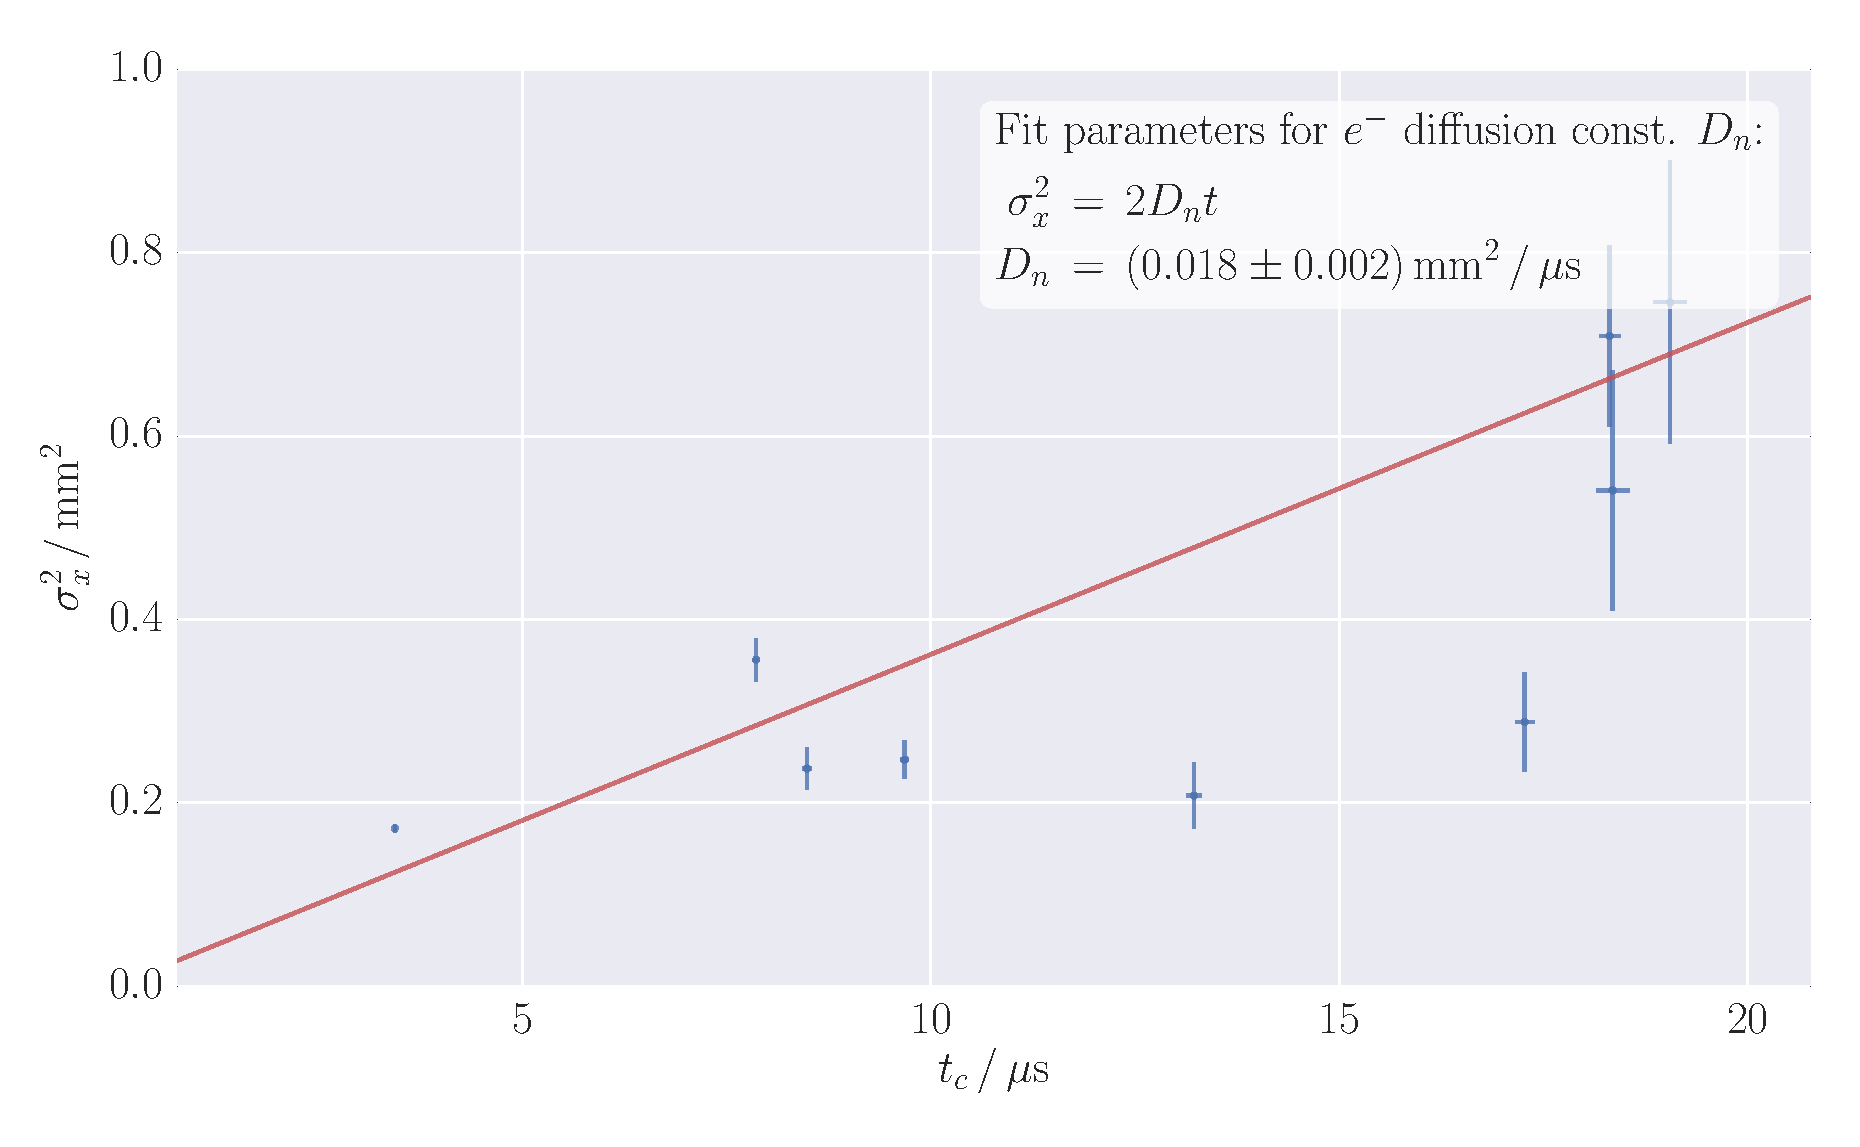
\includegraphics[width=1.0\textwidth]{figures/haynes_shockley_D_d}
    \caption{
        Spatial variances $\sigma_x^2$ fitted over center of gaussians $t_c$ 
        (corresponding to the time traveled by the distribution) with a linear 
        function in order to calculate the diffusion constant $D_n$ of electrons. 
        One clearly observes the strong disagreement of the obtained data and the 
        expectation. We refer to multiple sources of systematic errors and fluctuations 
        explaining this contrast. 
        }
    \label{fig:h_s_D_d}
\end{figure}
\FloatBarrier

\subsubsection{Measuring at constant $U$}
The procedure of this part of the experiment is roughly the same as before. 
Instead of changing the distance, we change the applied acceleration voltage 
$U_mathrm{acc}$, while $d$ remains constant at $d = (4.1 \pm 0.5)\,$mm. 
The raw data and fitted gaussians are all displayed in the appendix,
\ref{sec:appendix_h_s_plots_U}. A summary of the calculated parameters is 
again given in a table (\ref{tab:h_s_fit_parameters_U}). 
\renewcommand{\arraystretch}{1.5}
\begin{table}[htdp]
    \centering
    \caption{
        Results of fits with gaussians for all used data sets with variating 
        acceleration voltage
        $U_\mathrm{acc}$. Again, the $\chi^2$-tests are quite high due to 
        large scale fluctuations and noise. 
        }
    	\begin{tabular}{|p{2cm}|p{3cm}|p{3cm}|p{3cm}|p{2cm}|}
		\hline
		\rowcolor{tabcolor}
		$U_\mathrm{acc} \, / \, \mathrm{V}$        & $A \, / \, \mathrm{\frac{mm}{\mu s}}$ & 
     			$t_c \, / \, \mathrm{\mu s}$    & $\sigma_t \, / \, \mathrm{\mu s}$ & 
     			$\chi^2 / n_d$ \\ \hline
		$24.4$ & $2.6 \pm 0.3$ & $371.66 \pm 0.20$ & $1.82 \pm 0.20$ & $2.3$\\ 
		$32.8$ & $3.8 \pm 0.1$ & $368.12 \pm 0.04$ & $1.09 \pm 0.04$ & $9.0$\\ 
		$39.6$ & $2.4 \pm 0.2$ & $370.18 \pm 0.16$ & $1.50 \pm 0.16$ & $2.4$\\ 
		$41.2$ & $7.9 \pm 0.2$ & $366.72 \pm 0.03$ & $1.15 \pm 0.03$ & $115.0$\\ 
		$44.4$ & $8.0 \pm 0.3$ & $367.85 \pm 0.07$ & $1.55 \pm 0.08$ & $5.1$\\ 
		$46.4$ & $3.5 \pm 0.1$ & $368.25 \pm 0.04$ & $0.99 \pm 0.04$ & $9.1$\\ 
		$48.0$ & $4.3 \pm 0.2$ & $367.52 \pm 0.05$ & $1.08 \pm 0.05$ & $14.6$\\ 
		$48.4$ & $7.4 \pm 0.2$ & $366.68 \pm 0.03$ & $1.29 \pm 0.03$ & $10.3$\\ 
		$49.6$ & $7.3 \pm 0.1$ & $367.20 \pm 0.02$ & $1.40 \pm 0.03$ & $39.0$\\ 
		\hline
	\end{tabular}

    \label{tab:h_s_fit_parameters_U}
\end{table}

All fitted gaussians are displayed in figure%
~\ref{fig:h_s_all_gauss_U}. The expected distribution of descending amplitudes 
and enlarging widths is only partially observed -- a fact that will impede the 
further analysis. 
\begin{figure}
    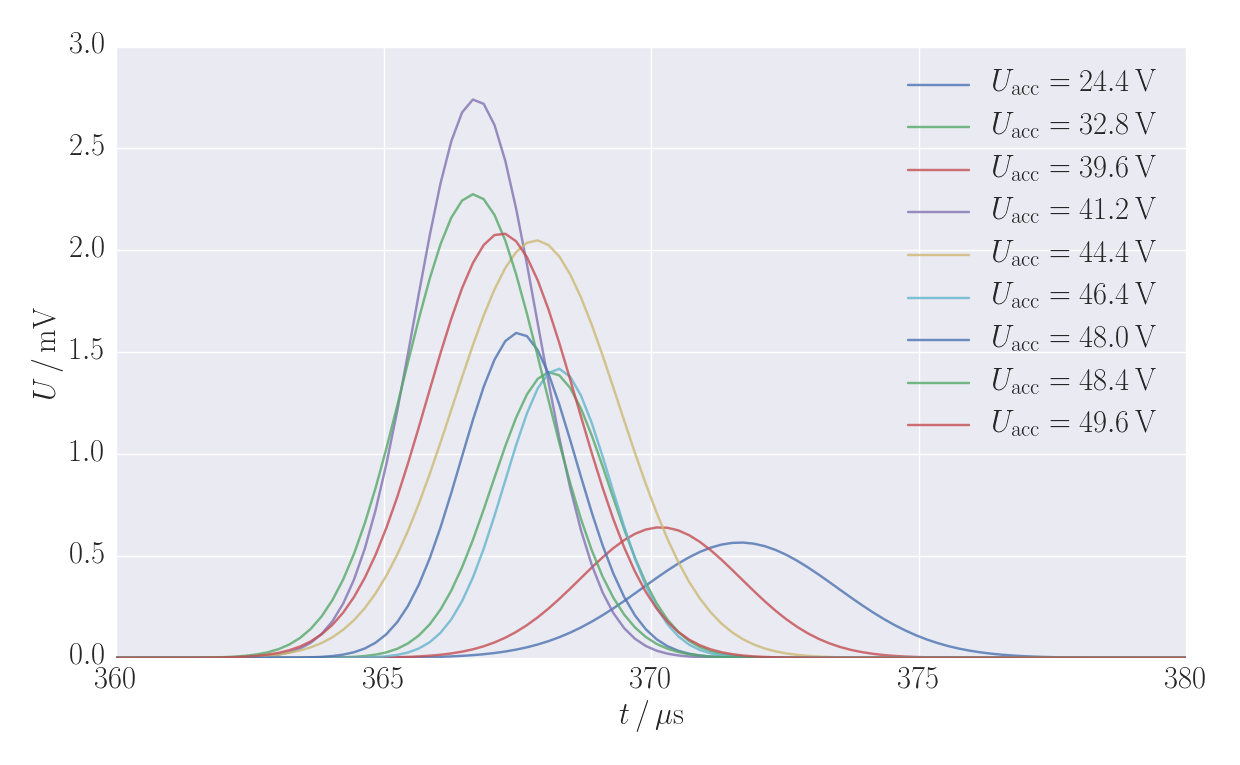
\includegraphics[width=1.0\textwidth]{figures/haynes_shockley_all_gauss_U}
    \caption{
        Fitted gaussian for constant $d$, variating the acceleration voltage 
        $U_\mathrm{acc}$. From the theory, one would expect the amplitudes to decline with 
        time $t$, while the distribution would get wider. This feature is only 
        partially given in our data. 
        }
    \label{fig:h_s_all_gauss_U}
\end{figure}
In order to get the linear correspondence between temporal and 
spatial center of the distribution, $t_c$ and $x_c$, we 
exchange one term of the defining equation \eqref{eq:x_c} and get 
\begin{equation}
    \frac{x_c}{E} = \mu_n t \, .
\end{equation}
With $x_c = d$ and $E = U_\mathrm{acc} / l$, we apply a fit of the form
\begin{equation}
    \frac{d \, l}{U_\mathrm{acc}} = \mu_n (t - t_0) \, ,
\end{equation}
where $t_0$ refers to the offset in time we observed. The result 
is shown in figure~\ref{fig:h_s_mu_e_U}. Although the fit is clearly underfed, 
as fluctuations of the observable magnitude would require a much larger 
set of data, we continue the calculation with the obtained parameters. 
Here, the electron mobility is directly calculated with 
\begin{equation}
    \begin{split}
        \mu_e   = (0.30 \pm 0.12)\, \mathrm{\frac{mm^2}{V\mu s}} \\
                = (3000 \pm 120)\, \mathrm{\frac{cm^2}{V\,s}} \,.
    \end{split}
\end{equation}
The value again lies notably below the accepted value. It does agree 
with the value measured in the first experiment within three standard deviations, 
which at least indicates the consistency of the results. 
\begin{figure}
    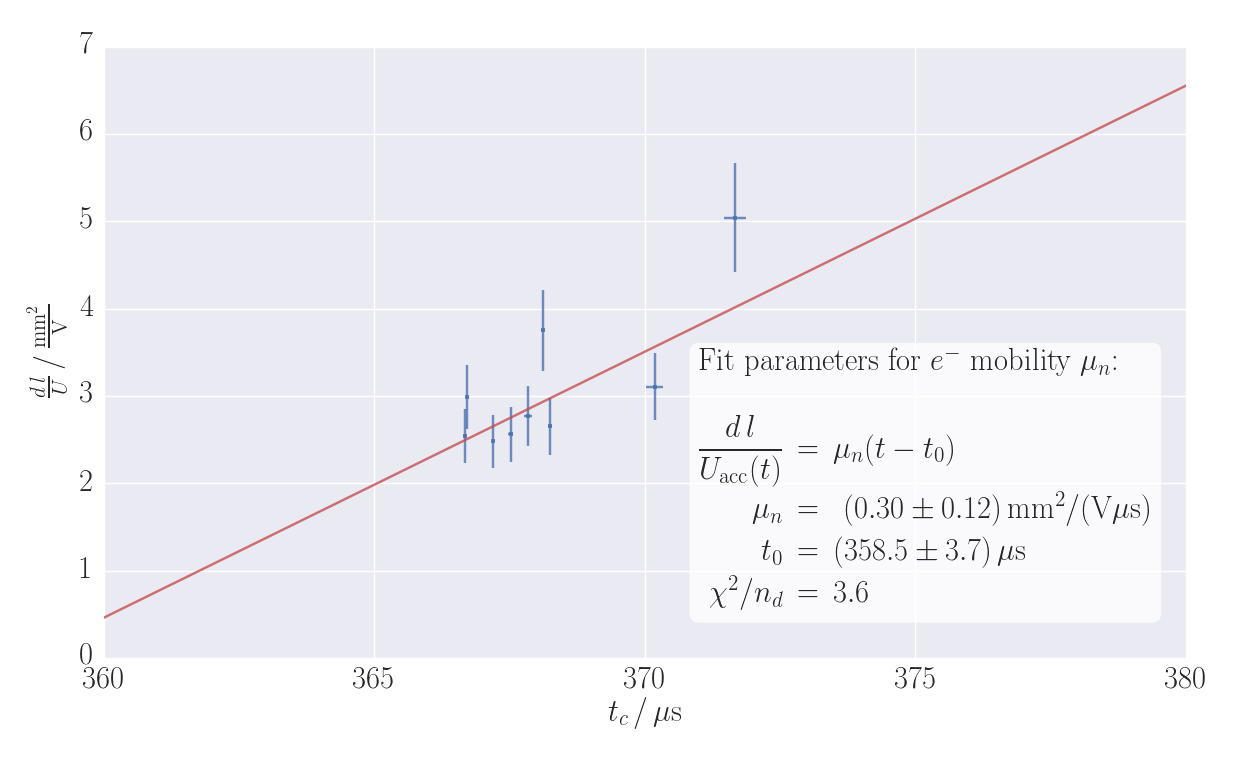
\includegraphics[width=1.0\textwidth]{figures/haynes_shockley_mu_e_U}
    \caption{
        Fitted straight line on centers of gaussians for constant $d$.  
        The little number of data points does not allow for a good fit. 
        Further, the errors obtained from fitting the gaussians do not
        capture the real errors, which might further be due to 
        fluctuations. This is also indicated by the $\chi^2$-test.
        }
    \label{fig:h_s_mu_e_d}
\end{figure}
We continue calculating the life time $\tau_n$, applying the 
transformation of the amplitude $C' = C / (\mu_n E)$. The resulting 
parameters together with the fit on the obtained data points is shown 
in figure~\ref{fig:h_s_tau_U}, yielding a life time of 
\begin{equation}
    \tau_n = (1.6 \pm 0.5)\, \mathrm{\mu s} \, .
\end{equation}
This parameter is in the same order of magnitude as the one obtained 
by the first measurement, but smaller and thus ever further away from 
the literature value. The discussion done before applies here as well. 
\begin{figure}
    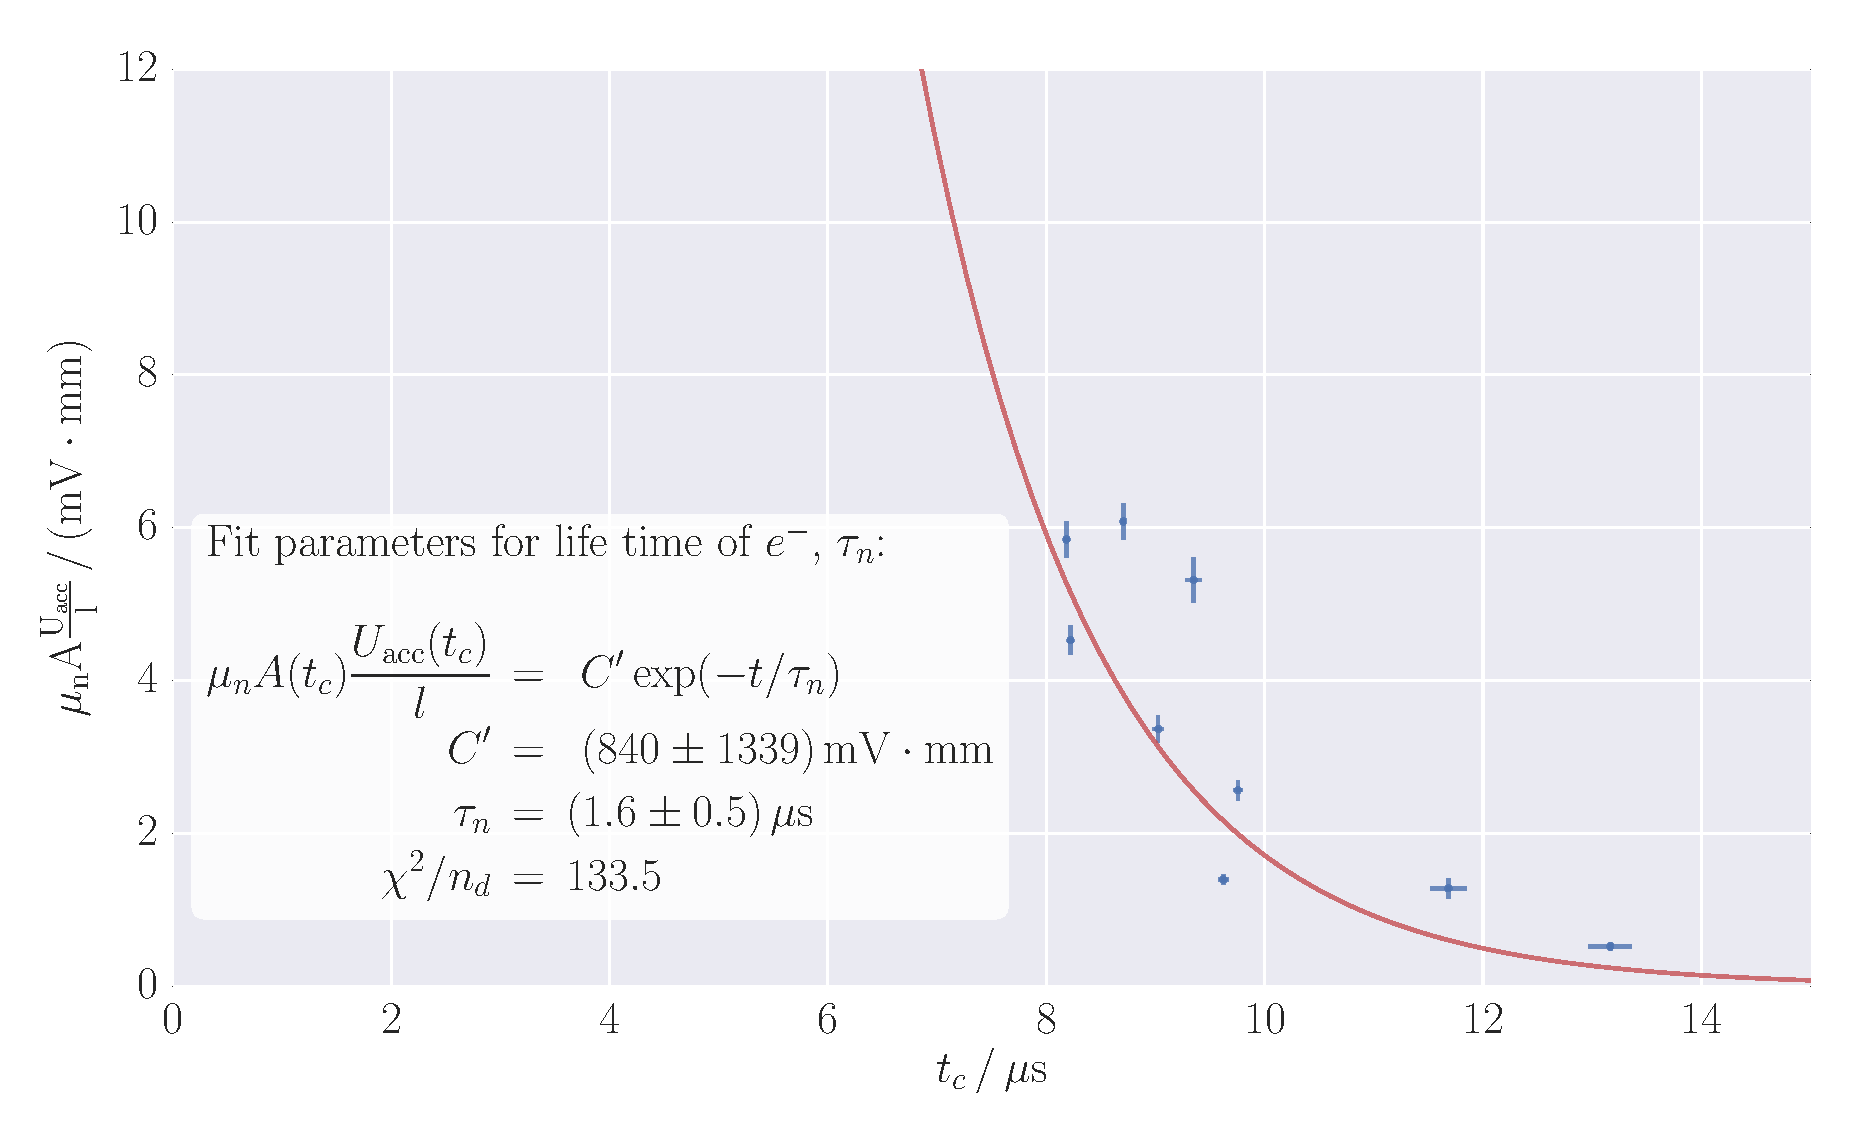
\includegraphics[width=1.0\textwidth]{figures/haynes_shockley_tau_U}
    \caption{
        Exponential fit to calculate the life time of free electrons in germanium. 
        The errors, stemming from the fit of gaussians on the original data, 
        are much to small, since they do not capture global fluctuations induced 
        by systematic errors. The resulting physical parameter $\tau_n$ should 
        thus be interpreted with care, using it as an approximation of the 
        order of magnitude. 
        }
    \label{fig:h_s_tau_U}
\end{figure}
The third and last calculation of this part of the experiment is the fit over the 
variances which are obtained analogously to the ones before by applying the 
described transformation from temporal to spatial quantities. 
In this case, however, the electron velocity is dependent on 
the voltage, yielding a different transformation for each $\sigma_t$. 
We will not further show intermediate steps of the transformations and 
plot only the resulting data with fits, see figure~\ref{fig:h_s_D_U}. 
The resulting fitted parameter of 
\begin{equation}
    D_n = (130 \pm 20)\, \mathrm{\frac{cm^2}{s}} 
\end{equation}
resembles the one measured before quite well. Considering the 
strong variance and low quality of the fit, this rather seems to 
be coincidental and should by no means obscure the large uncertainty 
and underestimation of the error due to systematical errors. 
\begin{figure}
    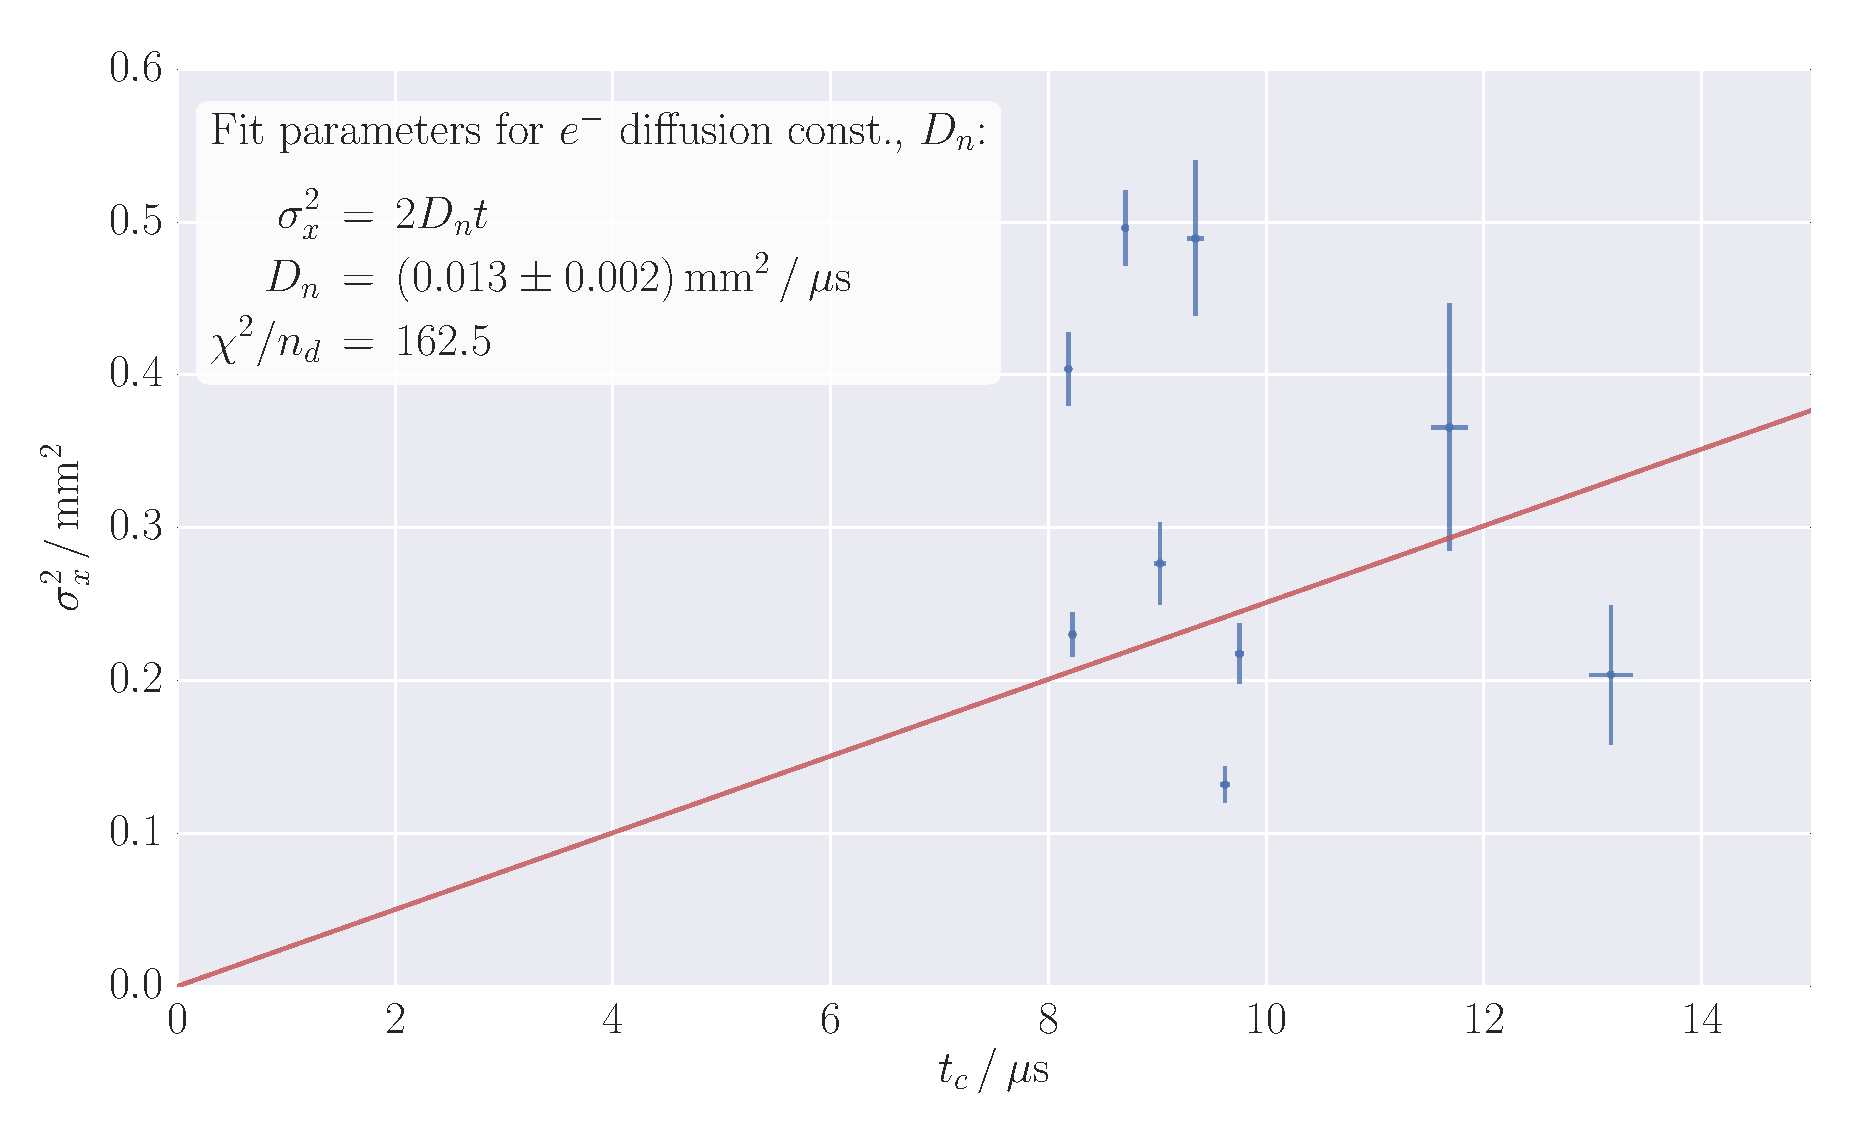
\includegraphics[width=1.0\textwidth]{figures/haynes_shockley_D_U}
    \caption{
        Linear fit through spatial variances $\sigma_x^2$. 
        The data does not seem to follow a linear behavior. 
        The usability of the result to assess the order of magnitude 
        of $D_n$ stems from the constraint of $\sigma_x^2(t = 0) = 0$, 
        has to be used very conservatively, though. The error 
        is only realistic if the constraint is taken as fixed -- 
        a non-zero variance for $t = 0$ would allow a much wider range of
        linear fits and thus a much higher uncertainty. 
        }
    \label{fig:h_s_D_U}
\end{figure}

\FloatBarrier

\subsection{Semiconductor detectors}
The measurement were done without any notable incidences, since 
the entire setup is automatized. We saved four data sets:
One for each combination of sample and detector. Due to time constraints, 
the background was not recorded. 

For each data set, we fitted gaussians according to the peaks expected:
For the $\,^{57}$Co sample, we expected two peaks at the right end of a somewhat 
broader distribution of counts with the left one (the 122.06 keV peak) being much higher
then the second (136.47 keV). For the $\,^{241}$Am sample, we expect one peak of 59.5 keV 
(thus roughly at half distance between zero and the $\,^{57}$Co peaks). 
The raw data and fitting is displayed in the panels \ref{fig:detector_CdTe}, 
\ref{fig:detector_Si}.
The fit parameters are listed in the plots. We refrain from stating the entire covariance 
matrices as all further calculations are done with one of the fitted parameters 
each (with the exception of the correspondence energy--channel, which generates new 
errors by linear fitting, loosing the information about correlation). 
The cobalt sample was not very active%
\footnote{an experience we already made during the experiment "short half lives"} 
such that the peak especially for the Si detector had to be done with a very low 
number of data. To be able to observe any signal at all, we rebinned the data 
by using the mean of two successive bins for this data set. In order to have let 
the algorithm converge, we entered initial guesses manually. An experimenting 
with changing initial guesses showed show stability, though . This is not documented 
since we consider the numerical stability of the used algorithms to be 
out of scope. The result of the fitting is, however, very much dependent on the 
range of channels selected to be fitted over. This range is indicated by
the curves of the fits plotted in the above figures. In general, we chose 
a longer range on the right side of each peak, as this side is 
much less influenced by additional underlying distributions. 
Physically, this observation corresponds to the losses during Compton 
scattering or other escaped electrons. In these cases, 
only a part of the entire energy of the initial photon stemming from the decay 
is absorbed by the detector. It is clear that these processes do not influence 
the right (higher energy) side of each peak, as long as overlapping with the next 
peak does not occur. 
\begin{figure}
    \centering
    \begin{subfigure}[b]{\pltw}
        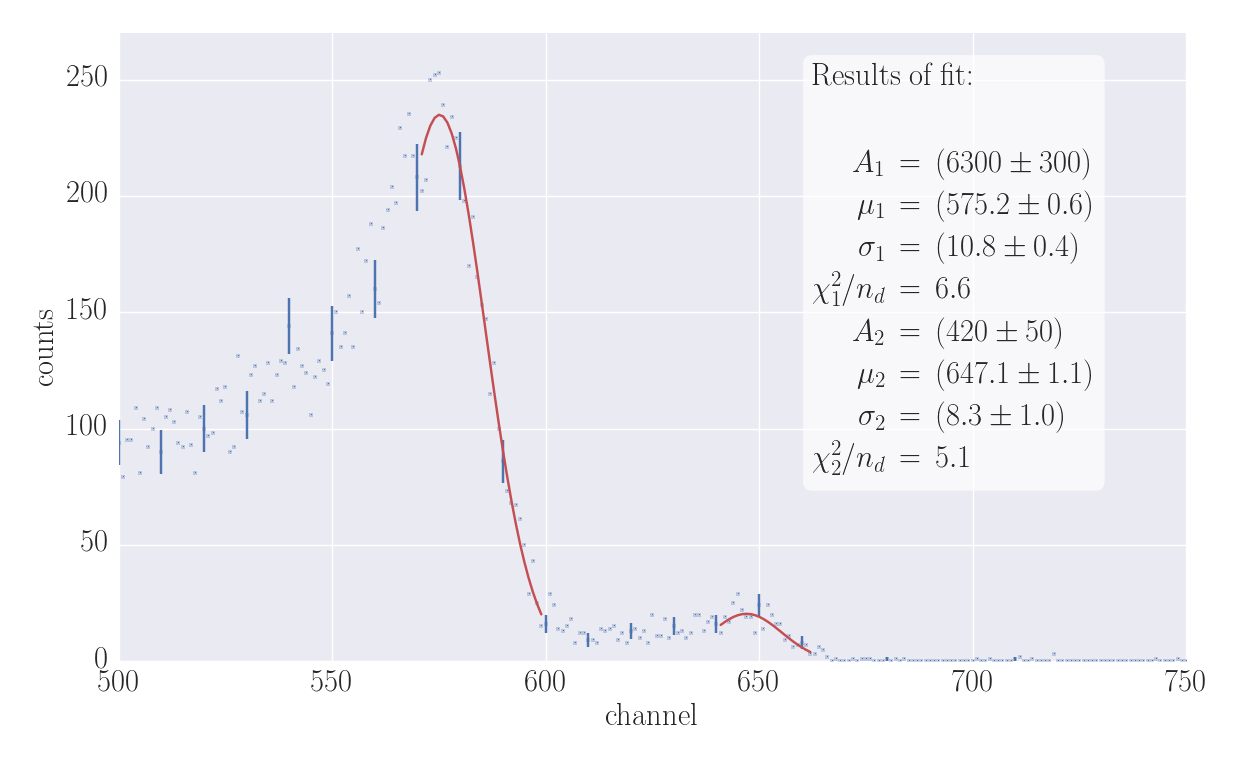
\includegraphics[width=1.0\linewidth]{figures/detector_Co_CdTe}
        \caption{}
        \label{fig:detector_Co_CdTe}
    \end{subfigure}
    \begin{subfigure}[b]{\pltw}
        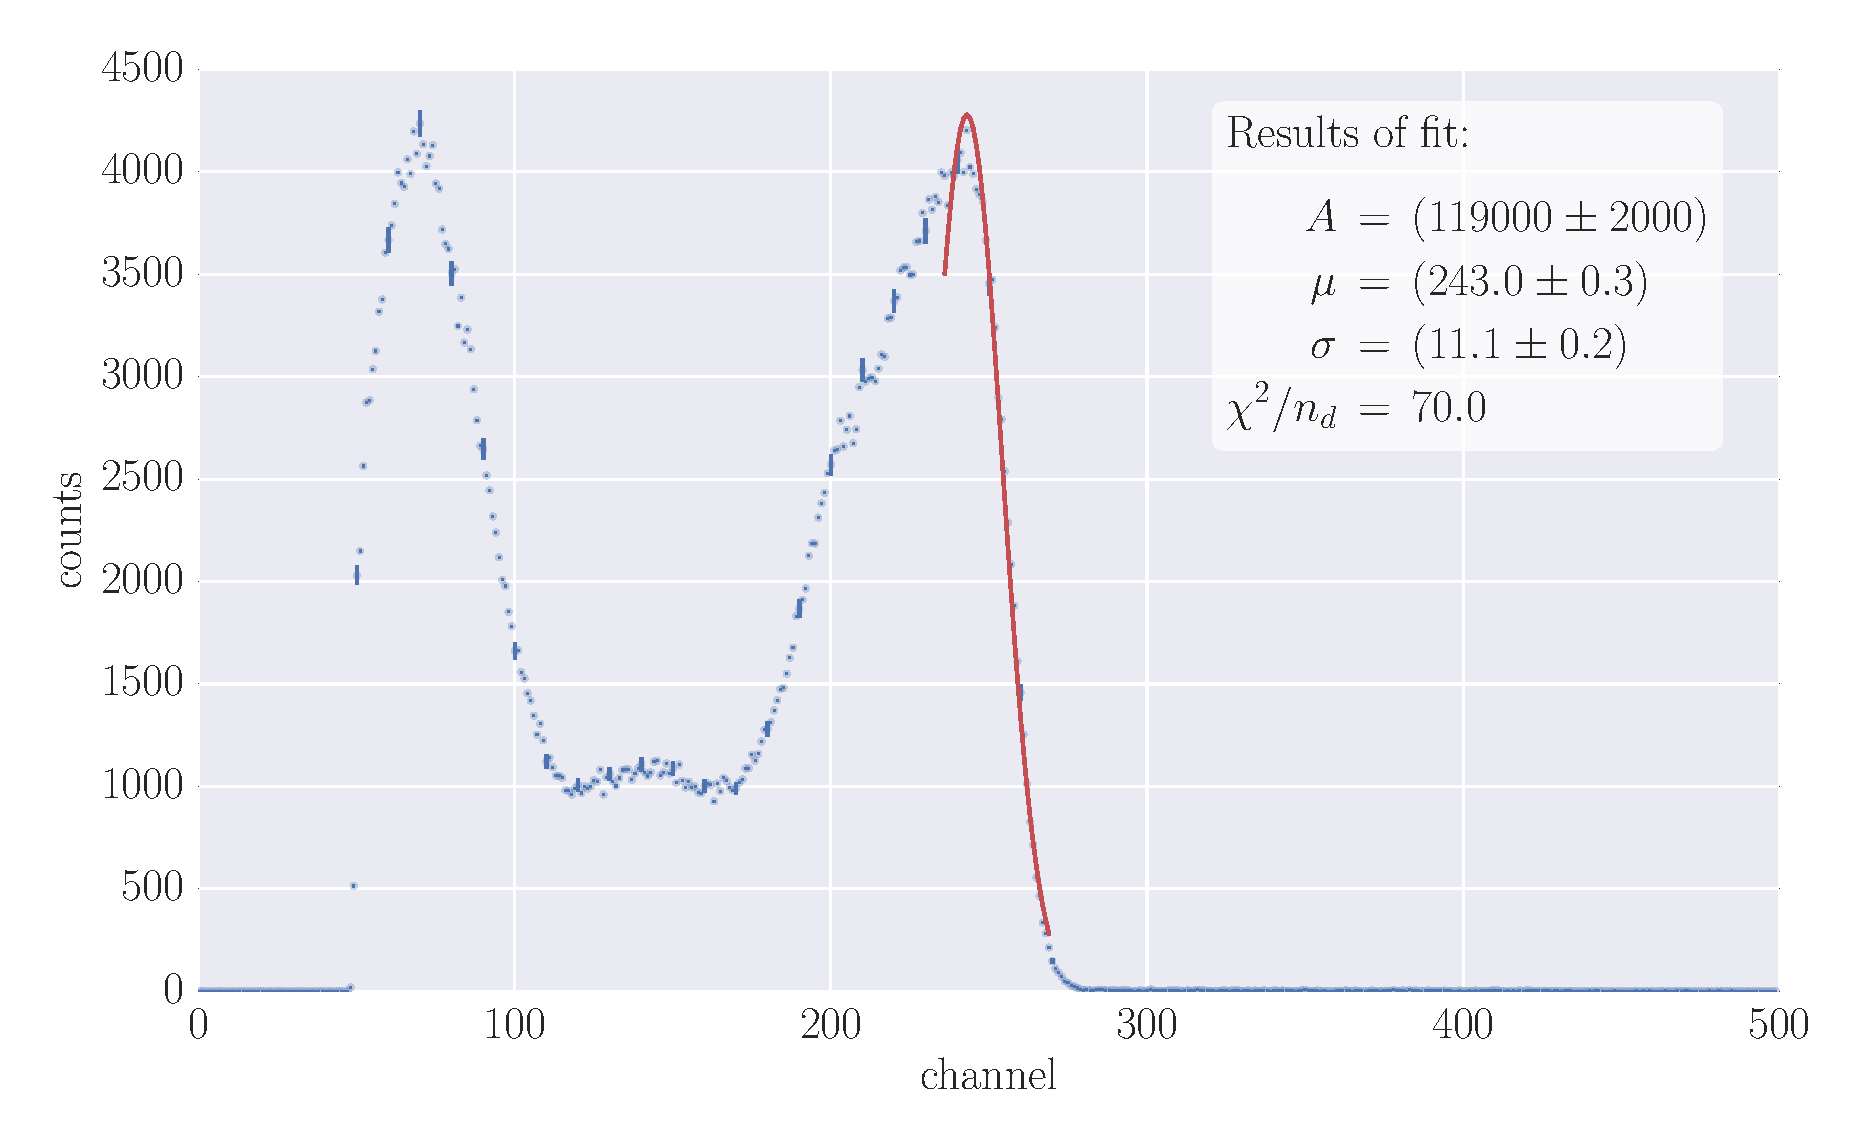
\includegraphics[width=1.0\linewidth]{figures/detector_Am_CdTe}
        \caption{}
        \label{fig:detector_Am_CdTe}
    \end{subfigure}
    \caption{
        Raw data obtained with CdTe detector as well as gaussians fitted 
        onto the expected peaks for the samples $^{57}$Co (\ref{fig:detector_Co_CdTe})
        and $^{241}$Am (\ref{fig:detector_Am_CdTe}). To maintain readability, the error bars 
        are only plotted for every tenth data point. The error is estimated as usual 
        with $\sqrt{N}$, the estimator for random variables following Poisson's distribution. 
        }
    \label{fig:detector_CdTe}
\end{figure}

\begin{figure}
    \centering
    \begin{subfigure}[b]{\pltw}
        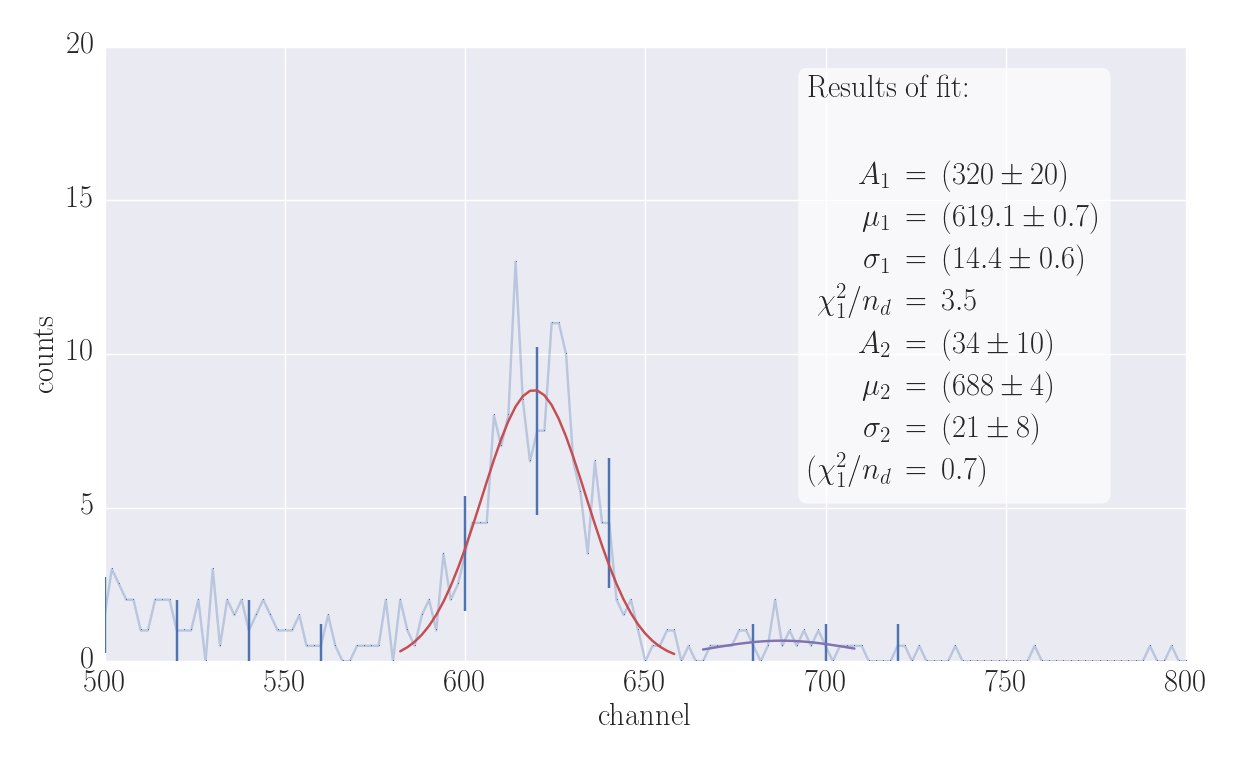
\includegraphics[width=1.0\linewidth]{figures/detector_Co_Si}
        \caption{}
        \label{fig:detector_Co_Si}
    \end{subfigure}
    \begin{subfigure}[b]{\pltw}
        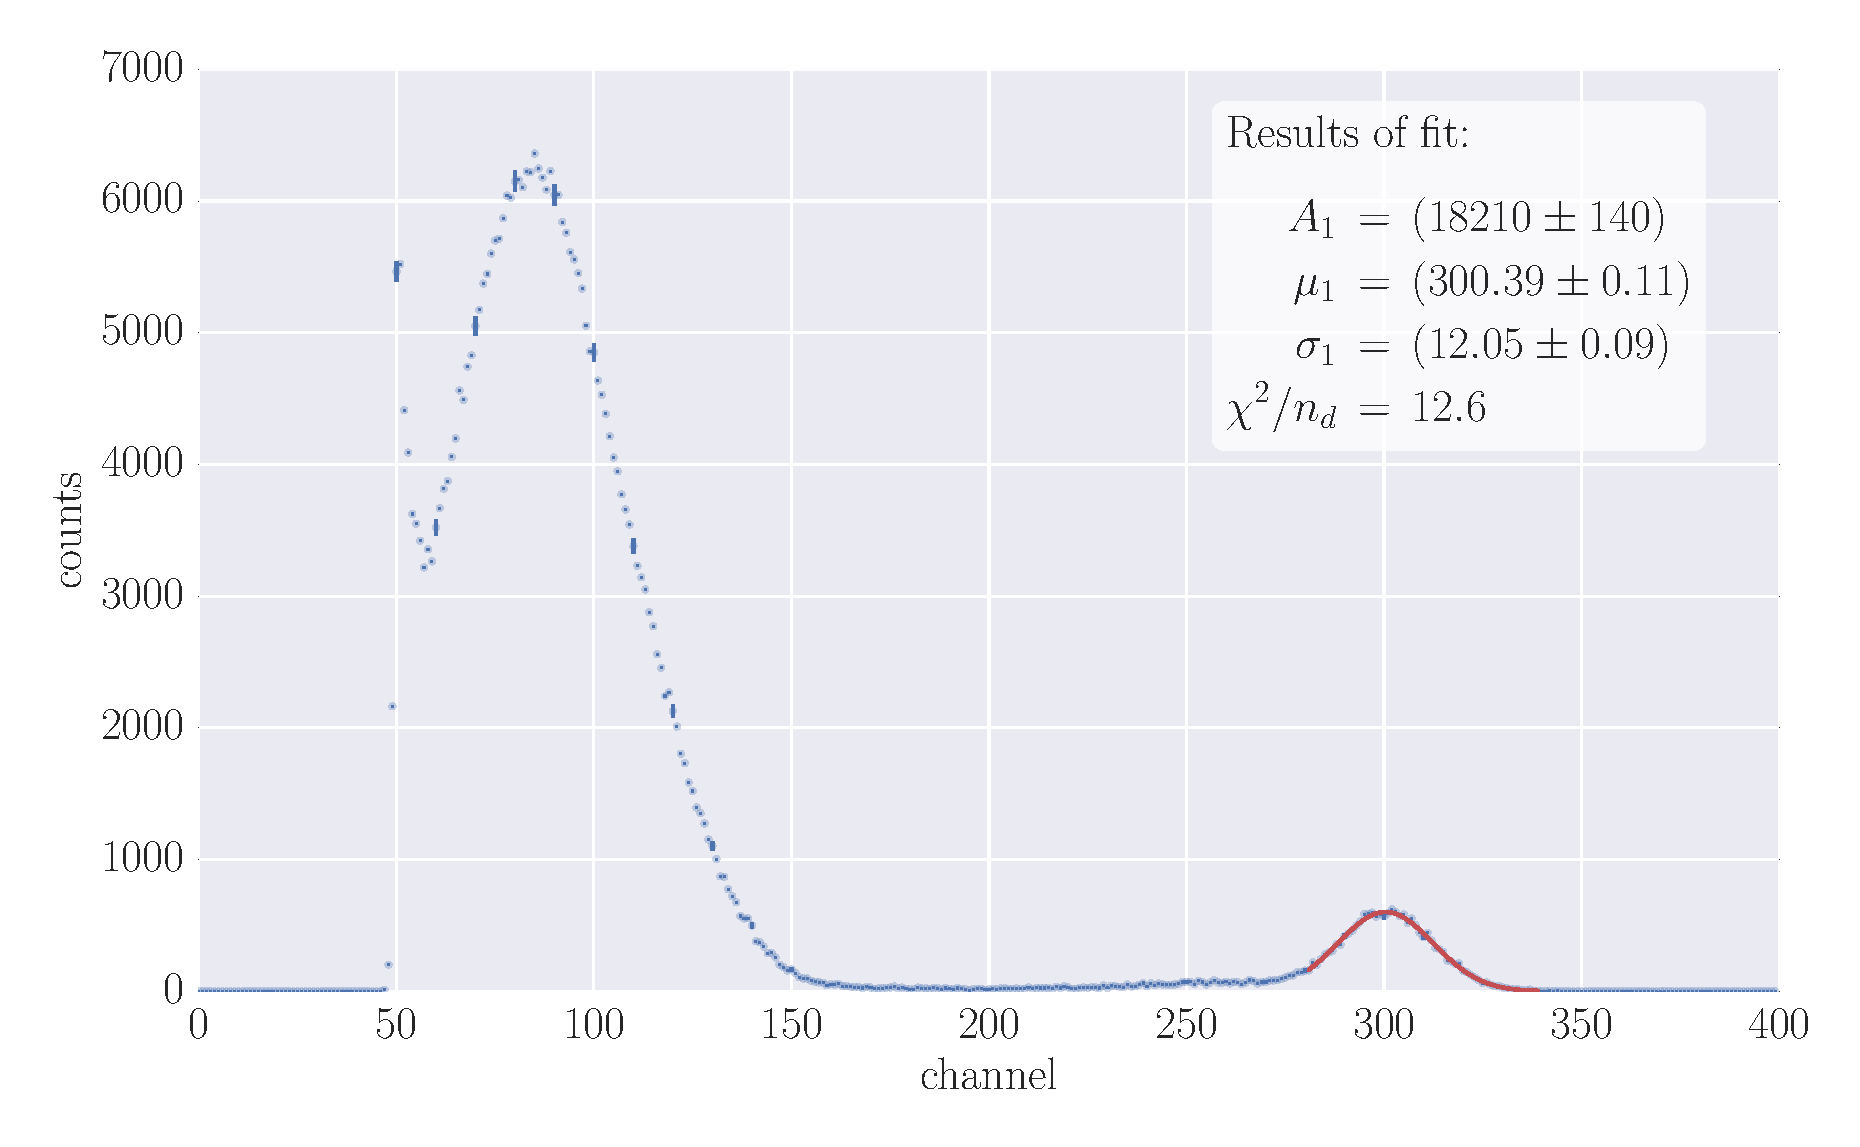
\includegraphics[width=1.0\linewidth]{figures/detector_Am_Si}
        \caption{}
        \label{fig:detector_Am_Si}
    \end{subfigure}
    \caption{
        Raw data obtained with CdTe detector as well as gaussians fitted 
        onto the expected peaks for the samples $^{57}$Co (\ref{fig:detector_Co_CdTe})
        and $^{241}$Am (\ref{fig:detector_Am_CdTe}). The data in the upper plot is rebinned 
        in order to obtain a visible peak.
        }
    \label{fig:detector_Si}
\end{figure}

We take the obtained centers $\mu$ of the distributions to do the calibration, 
i.~e. a linear fit of the form 
\begin{equation}
    E(\mu) = a \mu + E_0 \,
\end{equation}
in order to be able to associate an energy to each peak. The energies 
are taken from the know peaks as described before. The used data is shown in table 
\ref{tab:detector_peaks}, the linear interpolations are plotted in 
figures \ref{fig:detector_calibration}, found in the appendix. We get a linear coefficients
\begin{align}
    a_\mathrm{CdTe}  &=  (0.1890 \pm 0.0011)\, \mathrm{\frac{keV}{ch}}\, \\
    a_\mathrm{Si}  &=  (0.1964  \pm 0.0005)\, \mathrm{\frac{keV}{ch}} \, .
\end{align}
\begin{table}[htdp]
    \centering
    \caption{
        Peaks and corresponding energies for both semiconductors 
        and both samples. The values are used in the linear fit 
        in order to establish the relationship between channel 
        and energy.
        }
    	\begin{tabular}{|p{3cm}|p{3cm}|p{3cm}|p{3cm}|}
		\hline
		\rowcolor{tabcolor}
		Peak   & $E_\mathrm{peak}$ / keV & $\mathrm{\mu_{CdTe}}$ / Channel & $\mathrm{\mu_{Si}}$ / Channel\\ 
		\hline
		$^{241}\mathrm{Am}$ & $59.5$ & $243.0 \pm 0.3$ & $300.39 \pm 0.11$ \\ 
		$^{57}\mathrm{Co}_1$ & $122.06$ & $575.2 \pm 0.6$ & $619.1 \pm 0.7$ \\ 
		$^{57}\mathrm{Co}_2$ & $136.47$ & $647.1 \pm 1.1$ & $688 \pm 4$ \\ 
		\hline
	\end{tabular}

    \label{tab:detector_peaks}
\end{table}
Using these coefficients, we can calculate the relative energy resolution 
of the detectors. This is done applying the formulae discussed in the procedure 
section, see equation \eqref{eq:RER}. The transformation of the standard deviation 
and the resulting resolutions are displayed in table \ref{tab:detector_RER}. 
It turns out that the relative resolution of both detectors lies in the same 
order of magnitude, seeing notable difference only for the 136 keV $^{57}$Co peak.
One has to keep in mind that this peak was especially subject to uncertainties 
as the number of events was to small to do a realistic fit. Further, the Si 
detector has a slightly higher resolution for all tested energies. 
A yet more interesting result of this part of the analysis is, that 
the width of the peaks does not change notably with the energy, 
such that the relative resolution gets better with higher energies. 
In this case, it is about twice as high for the Am peak compared to 
that Co peak for both detectors. 
\begin{table}[htdp]
    \centering
    \caption{
        Relative energy resolutions of CdTe (upper) and 
        Si (lower) detector 
        for the three observed peaks, calculated from the 
        width of the fitted gaussians. 
        }
    	\begin{tabular}{|p{2cm}|p{2.5cm}|p{3cm}|p{3cm}|p{3cm}|}
		\hline
		\rowcolor{tabcolor}
		Peak   & $E_\mathrm{peak}$ / keV & $\sigma_\mathrm{CdTe}$ / Channel &             $\sigma_{E, \mathrm{CdTe}}$ /keV & $\mathrm{RER_{CdTe}}(E)$ \\ 
		\hline
		$^{57}\mathrm{Co}_1$ & $122.06$ & $10.8 \pm 0.4$ & $2.03 \pm 0.07$ & $0.0391 \pm 0.0014$\\ 
		$^{57}\mathrm{Co}_2$ & $136.47$ & $8.3 \pm 1.0$ & $1.6 \pm 0.2$ & $0.027 \pm 0.003$\\ 
		$^{241}\mathrm{Am}$ & $59.5$ & $11.1 \pm 0.2$ & $2.10 \pm 0.04$ & $0.083 \pm 0.002$\\ 
		\hline &&&&\\ 
		\hline
		\rowcolor{tabcolor}
		Peak   & $E_\mathrm{peak}$ / keV & $\sigma_\mathrm{Si}$ / Channel &             $\sigma_{E, \mathrm{Si}}$ /keV & $\mathrm{RER_{Si}}(E)$ \\ 
		\hline
		$^{57}\mathrm{Co}_1$ & $122.06$ & $10.8 \pm 0.4$ & $2.03 \pm 0.07$ & $0.0391 \pm 0.0014$\\ 
		$^{57}\mathrm{Co}_2$ & $136.47$ & $8.3 \pm 1.0$ & $1.6 \pm 0.2$ & $0.027 \pm 0.003$\\ 
		$^{241}\mathrm{Am}$ & $59.5$ & $11.1 \pm 0.2$ & $2.10 \pm 0.04$ & $0.083 \pm 0.002$\\ 
		\hline
	\end{tabular}

    \label{tab:detector_RER}
\end{table}
The crucial part of this experiment lies in analyzing the qualities 
of both semiconductors as detectors, which is quantitatively expressed 
by the absorption probability: In many occasions one wants to now the 
activity of a sample. In order to get reliable data, it is crucial to 
register as many emitted photons as possible -- thus a higher absorption 
coefficient indicates a better material for the according experiments. 
We expect the CdTe semiconductor to show a much higher absorption rate 
due to its higher mass density (which is a determining factor for the 
    cross section). 
\begin{table}[htdp]
    \centering
    \caption{
        Amplitudes $A$ obtained from the gaussian fits and 
        resulting absorption ratio between CdTe and Si detector 
        with the active areas $a_{Si} = 100\, \mathrm{mm^2}$ and 
        $a_{CdTe} = 23\, \mathrm{mm^2}$.
        }
    	\begin{tabular}{|p{3cm}|p{3cm}|p{3cm}|p{3cm}|}
		\hline
		\rowcolor{tabcolor}
		Peak   & $A_\mathrm{CdTe}$ & $A_\mathrm{Si}$ & $P$\\ 
		\hline
		$^{57}\mathrm{Co}_1$ & $6300 \pm 300$ & $320 \pm 20$ & $0.219 \pm 0.014$\\ 
		$^{57}\mathrm{Co}_2$ & $420 \pm 50$ & $34 \pm 10$ & $0.35 \pm 0.11$\\ 
		$^{241}\mathrm{Am}$ & $119000 \pm 2000$ & $18210 \pm 140$ & $0.664 \pm 0.014$\\ 
		\hline
	\end{tabular}

    \label{tab:detector_ratio}
\end{table}
The literature values~\cite{nist} for the energies under 
examination are given by 
\begin{align}
    \frac{A_\mathrm{Si}}{A_\mathrm{CdTe}}(59 \,\mathrm{keV}) &= 1.40 \% \\
    \frac{A_\mathrm{Si}}{A_\mathrm{CdTe}}(122 \,\mathrm{keV}) &= 1.83 \% \\
    \frac{A_\mathrm{Si}}{A_\mathrm{CdTe}}(136 \,\mathrm{keV}) &= 2.00 \%
\end{align}
The order of magnitude is correct in all cases, although 
errors obtained from propagation underestimate the 
real errors -- due to the low number of data as well as systematic 
errors introduced for example by the different losses. 
The obtained values do not quite show the expected behavior 
of rising absorption ratio for higher energies.
However, 
it is clear, that the CdTe has a much higher absorption coefficient and 
can thus be considered to be the better detector in this kind of 
experiment. 

\section{Conclusion}
In the first part of the experiment, we basically obtained one 
central results: The approximated band gap energy $E_g$ for germanium 
and silicon. Our measured values lie at 
\begin{align}
    E_{g, \mathrm{Si}} &= (1.14 \pm 0.05) \,\mathrm{eV} \\
    E_{g, \mathrm{Ge}} &= (0.69 \pm 0.03) \,\mathrm{eV}
\end{align}
Both values cover the literature values within one standard deviation.
This accuracy was a rather surprising result to us, as we expected the 
applied method to be of a much lower certainty. 

The values measured in the Haynes \& Shockley experiment 
are displayed in the table~\ref{tab:conc_h_s} below:
\renewcommand{\arraystretch}{1.5}
\begin{table}[H]
    \centering
    \caption{
        Results of the Haynes \& Shockley experiment, variating the 
        acceleration voltage or the distance between creating the 
        cloud of free charge and measuring it. The errors correspond 
        to propagated errors of fitting not including systematical ones 
        and are thus underestimated. 
        }
	\begin{tabular}{|p{4cm}|p{3cm}|p{3cm}|p{3cm}|}
		\hline
		\rowcolor{tabcolor}
		Parameter           & $U = \text{const.}$   & $d = \text{const.}$   & Literature~\cite{staatsexamen} \\ 
        \hline
        mobility $\mu_n$    & $2640 \pm 130$        & $3000 \pm 120$        & $3900$     \\
        life time $\tau_n$  & $6.7 \pm 1.0$         & $1.6 \pm 0.5$         & $45 \pm 2$ \\
        diffusion const. $D_n$ & $140 \pm 20$      & $130 \pm 20$          & $101$     \\
		\hline
	\end{tabular}
    \label{tab:conc_h_s}
\end{table}
For both the electron mobility and diffusion constant we observe agreement in the 
order of magnitude between our results and the given literature values. The 
errors are underestimated due to not including systematical errors in the calculation. 
Other the shortcomings of the electronics (which we experienced in terms 
of loosing the signal), it is clear that the experiment does not allow the 
measurement of these constants in a perfect crystal. This is especially 
true for the life time, which is one order of magnitude smaller then the 
accepted value for germanium. 

Examination of the two semiconductors Si and CdTe gave an insight into the 
characteristics that allow for the usage as detectors for ionizing 
radiation. The central result is the superiority of heavier materials
(here represented by CdTe) over light ones (Si) when the registration of as 
many events as possible is key. The quantitative result, 
the ratio of absorption coefficients has been estimated to be
\begin{align}
    \mathrm{\frac{Abs_{Si}}{Abs_{CdTe}}}(59.5\, \mathrm{keV}) &= (3.51 \pm 0.07) \\
    \mathrm{\frac{Abs_{Si}}{Abs_{CdTe}}}(122.06\, \mathrm{keV}) &= (1.16 \pm 0.08)\\ 
    \mathrm{\frac{Abs_{Si}}{Abs_{CdTe}}}(136.47\, \mathrm{keV}) &= (1.9 \pm 0.6) \, ,
\end{align}
agreeing with the literature values in order of magnitude. The errors 
are those obtained by numerical calculation and do not include 
systematical errors, such as impurities or errors induced by the electronics. 
With one setup and the two possible semiconductors as detectors, one 
would thus need to measure 30 to 60 times as long with the Si semiconductor 
to obtain the same number of counts and thus the same statistical error. 
As a second, somewhat less striking result, we calculated the 
relative energy resolution (RER). The main result here is the increasing 
resolution with increasing energy: The resolution at 122 keV Co peak is 
twice the one at the 59.5 keV Am peak for both semiconductors.  

All three experiments resulted in a good introduction into semiconductor physics. 
Especially the Haynes and Shockley experiment, notwithstanding the disagreement in 
numerical results, gave a nice insight into models of the reality in semiconductors. 


\cleardoublepage

\phantomsection

\addcontentsline{toc}{section}{Bibliography und List of figures}
\bibliographystyle{plain}
\bibliography{report}
\listoffigures

\section{Appendix: Handwritten records of the experiment}
\label{sec:appendix}
    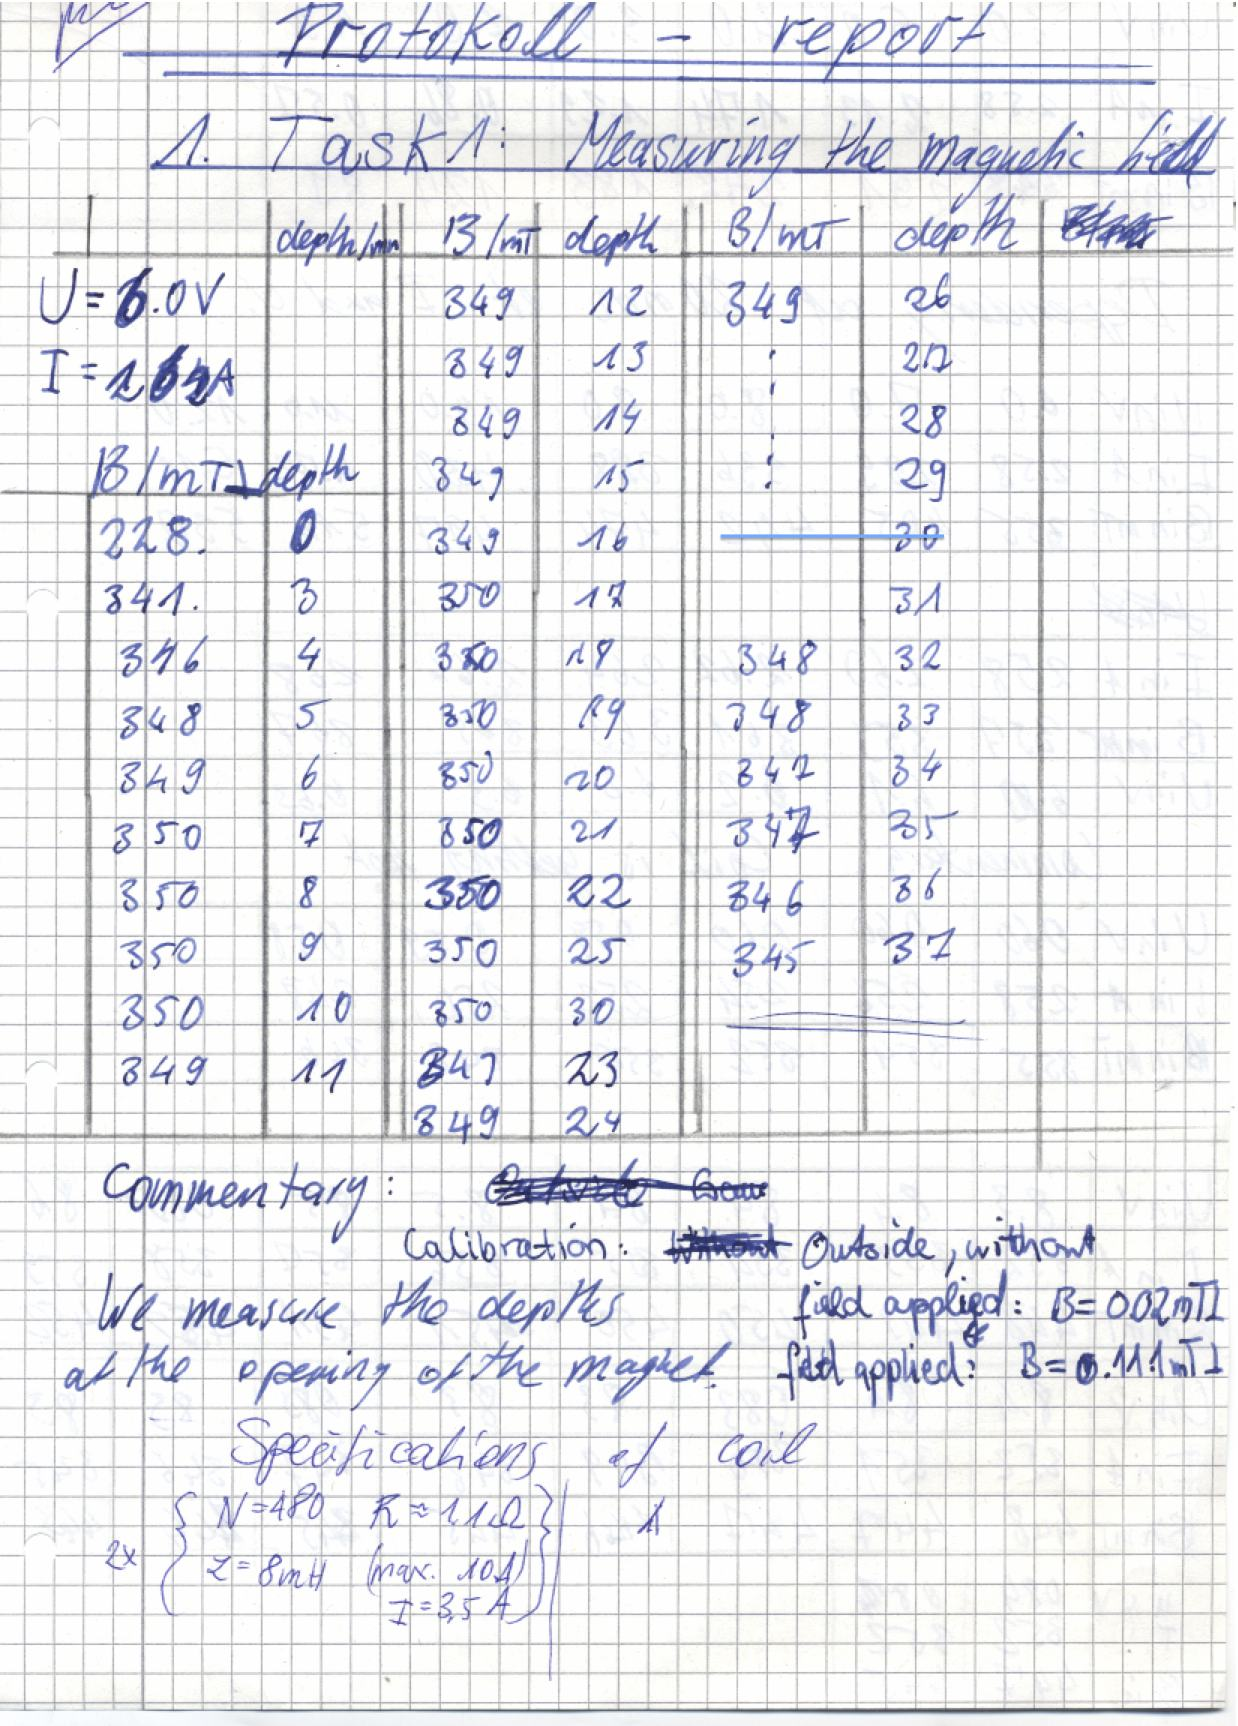
\includegraphics[width=\linewidth]{appendix/spin1.jpg}
\clearpage
    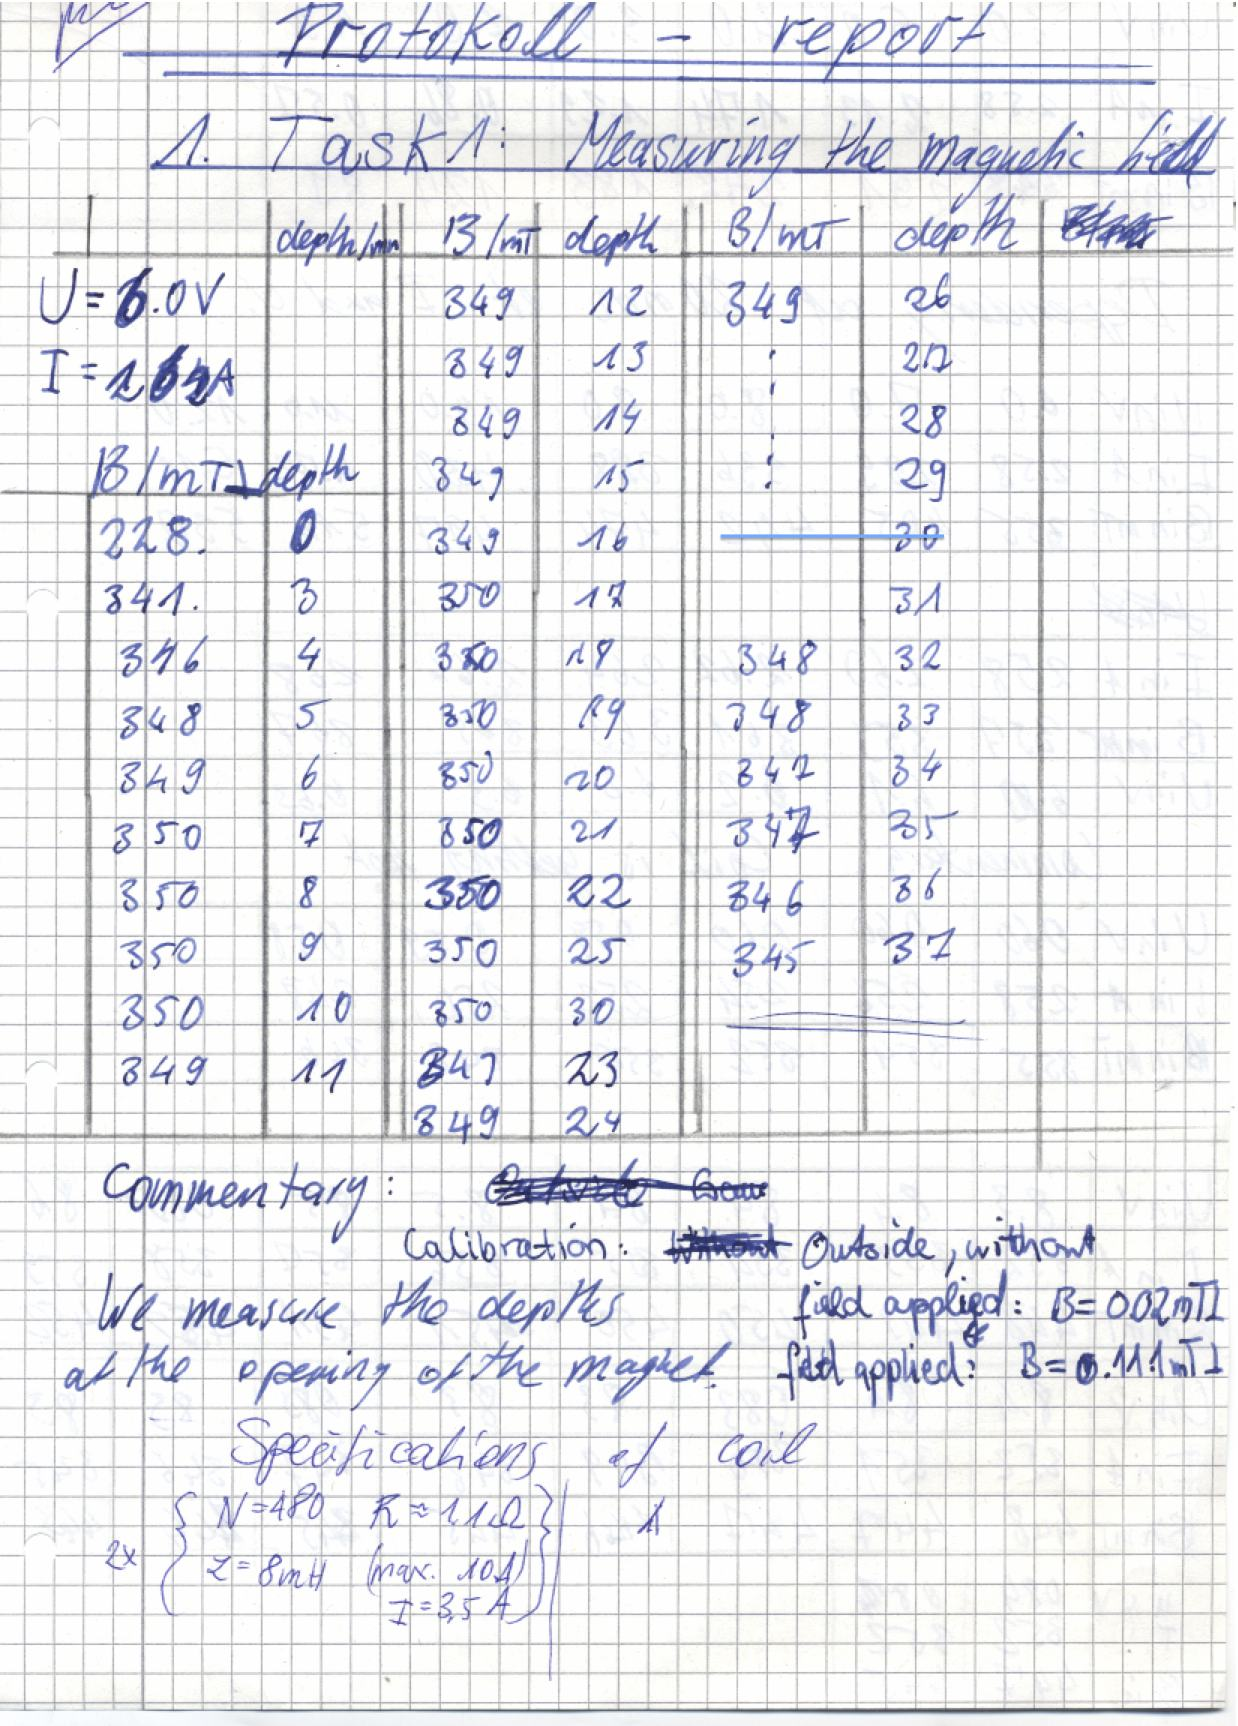
\includegraphics[width=\linewidth]{appendix/spin1.jpg}
\clearpage
    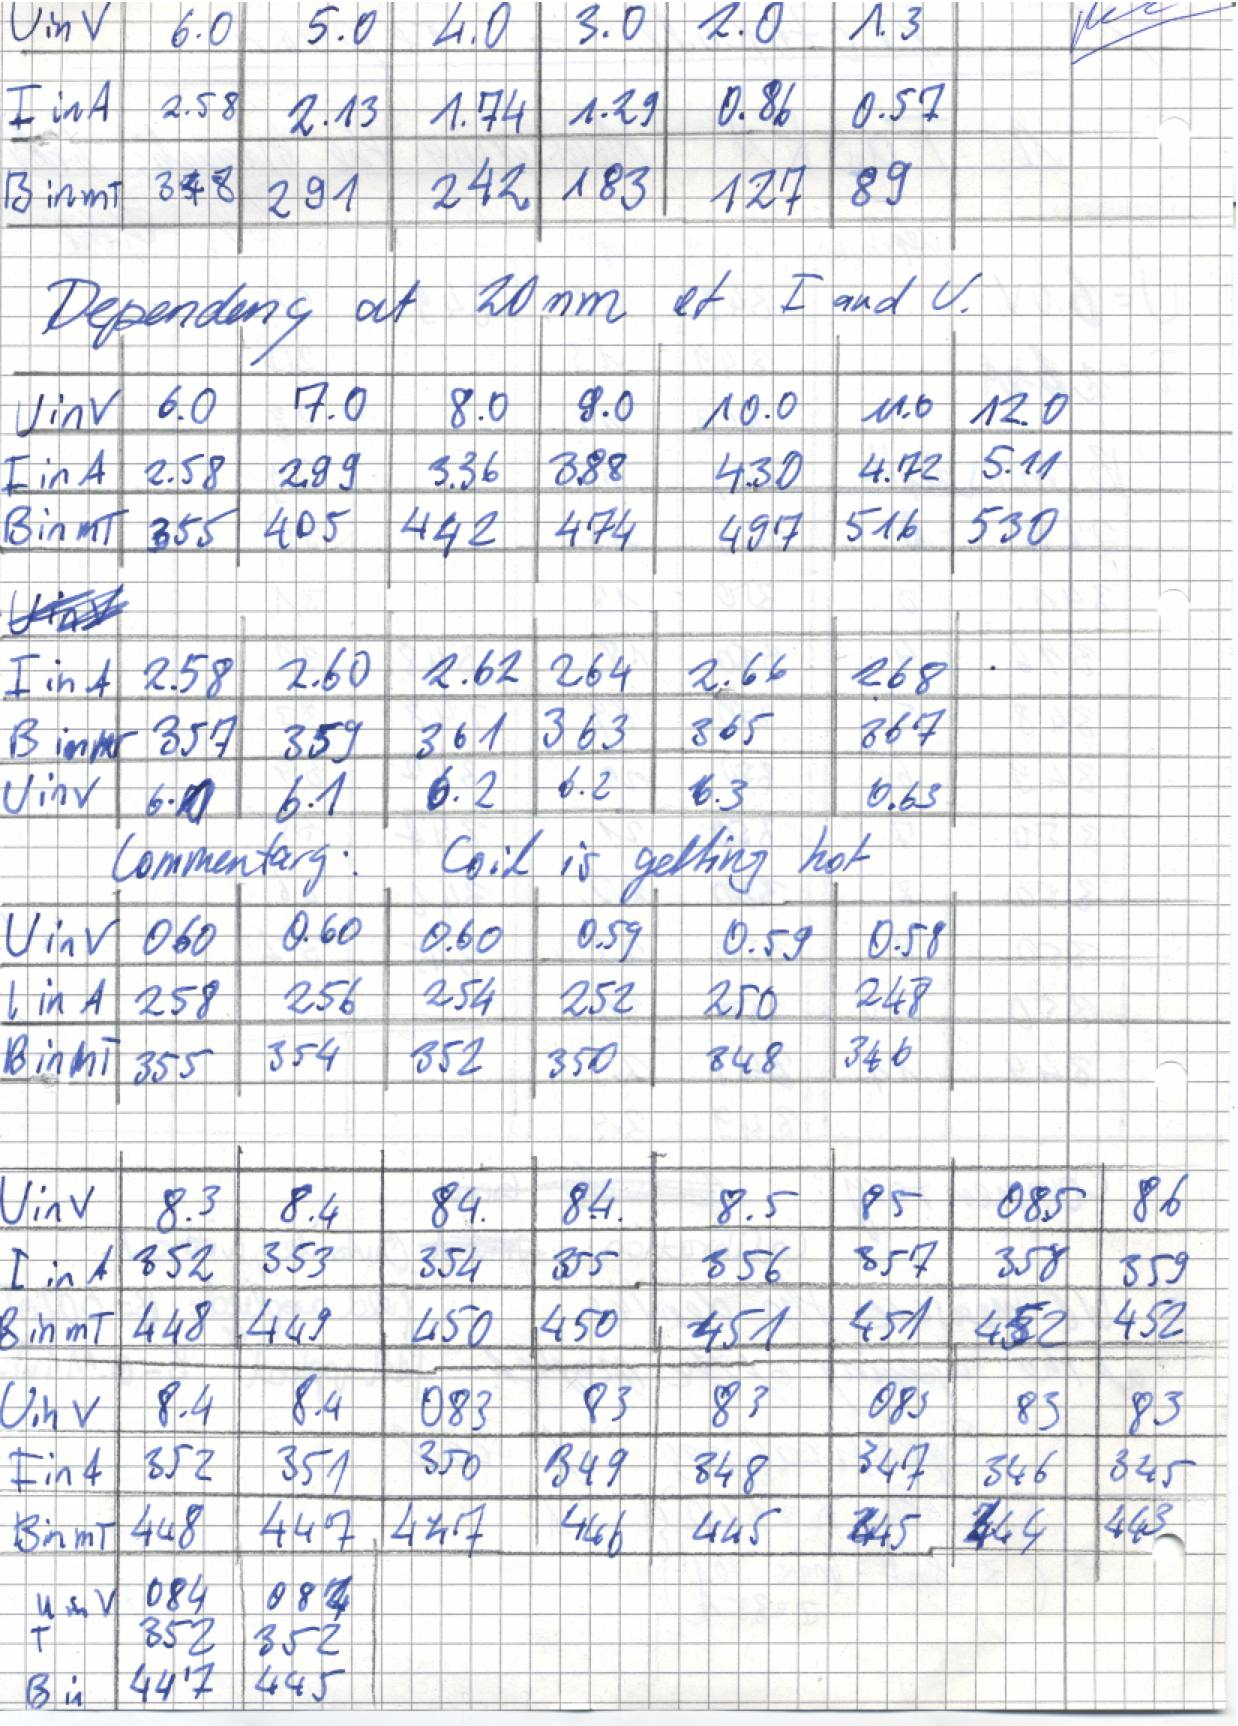
\includegraphics[width=\linewidth]{appendix/spin2.jpg}
\clearpage
    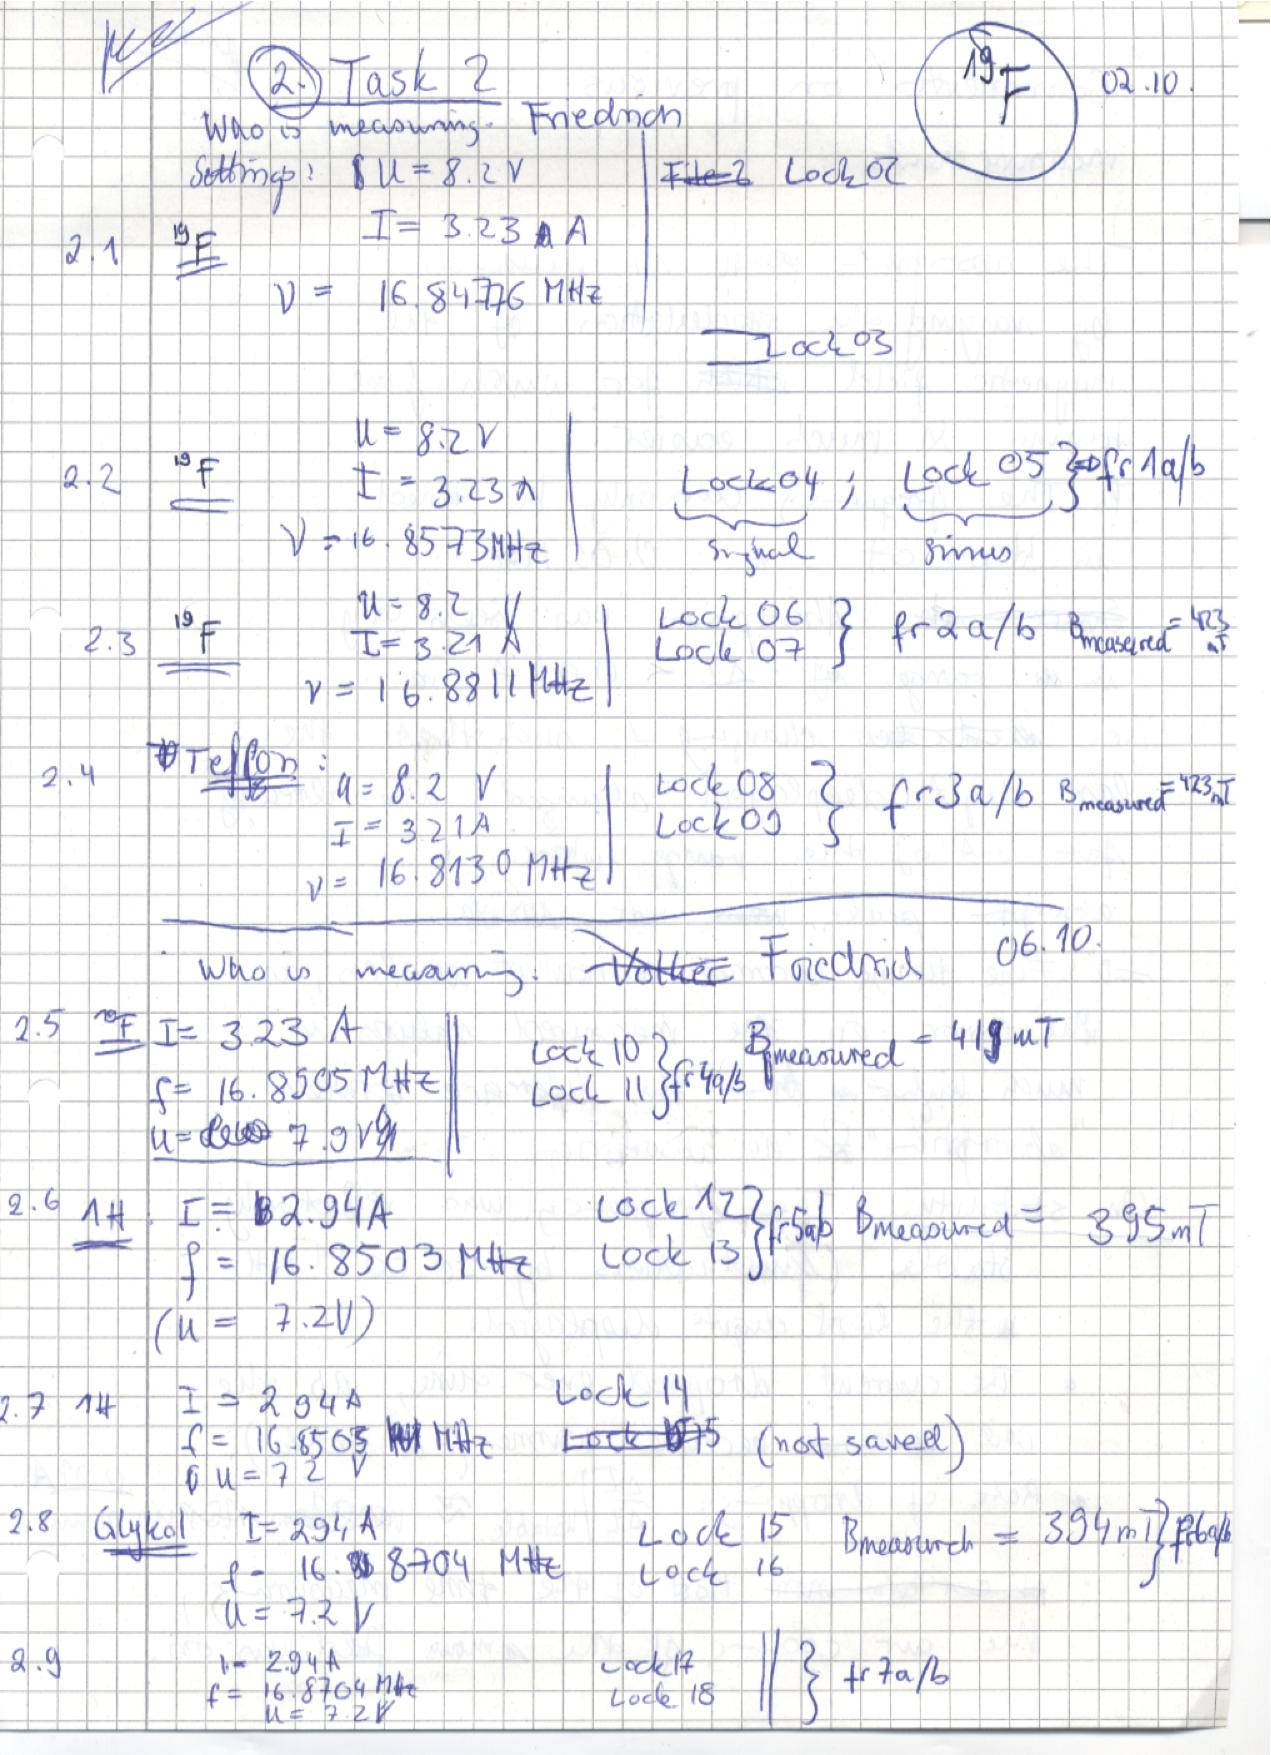
\includegraphics[width=\linewidth]{appendix/spin3.jpg}
\clearpage
    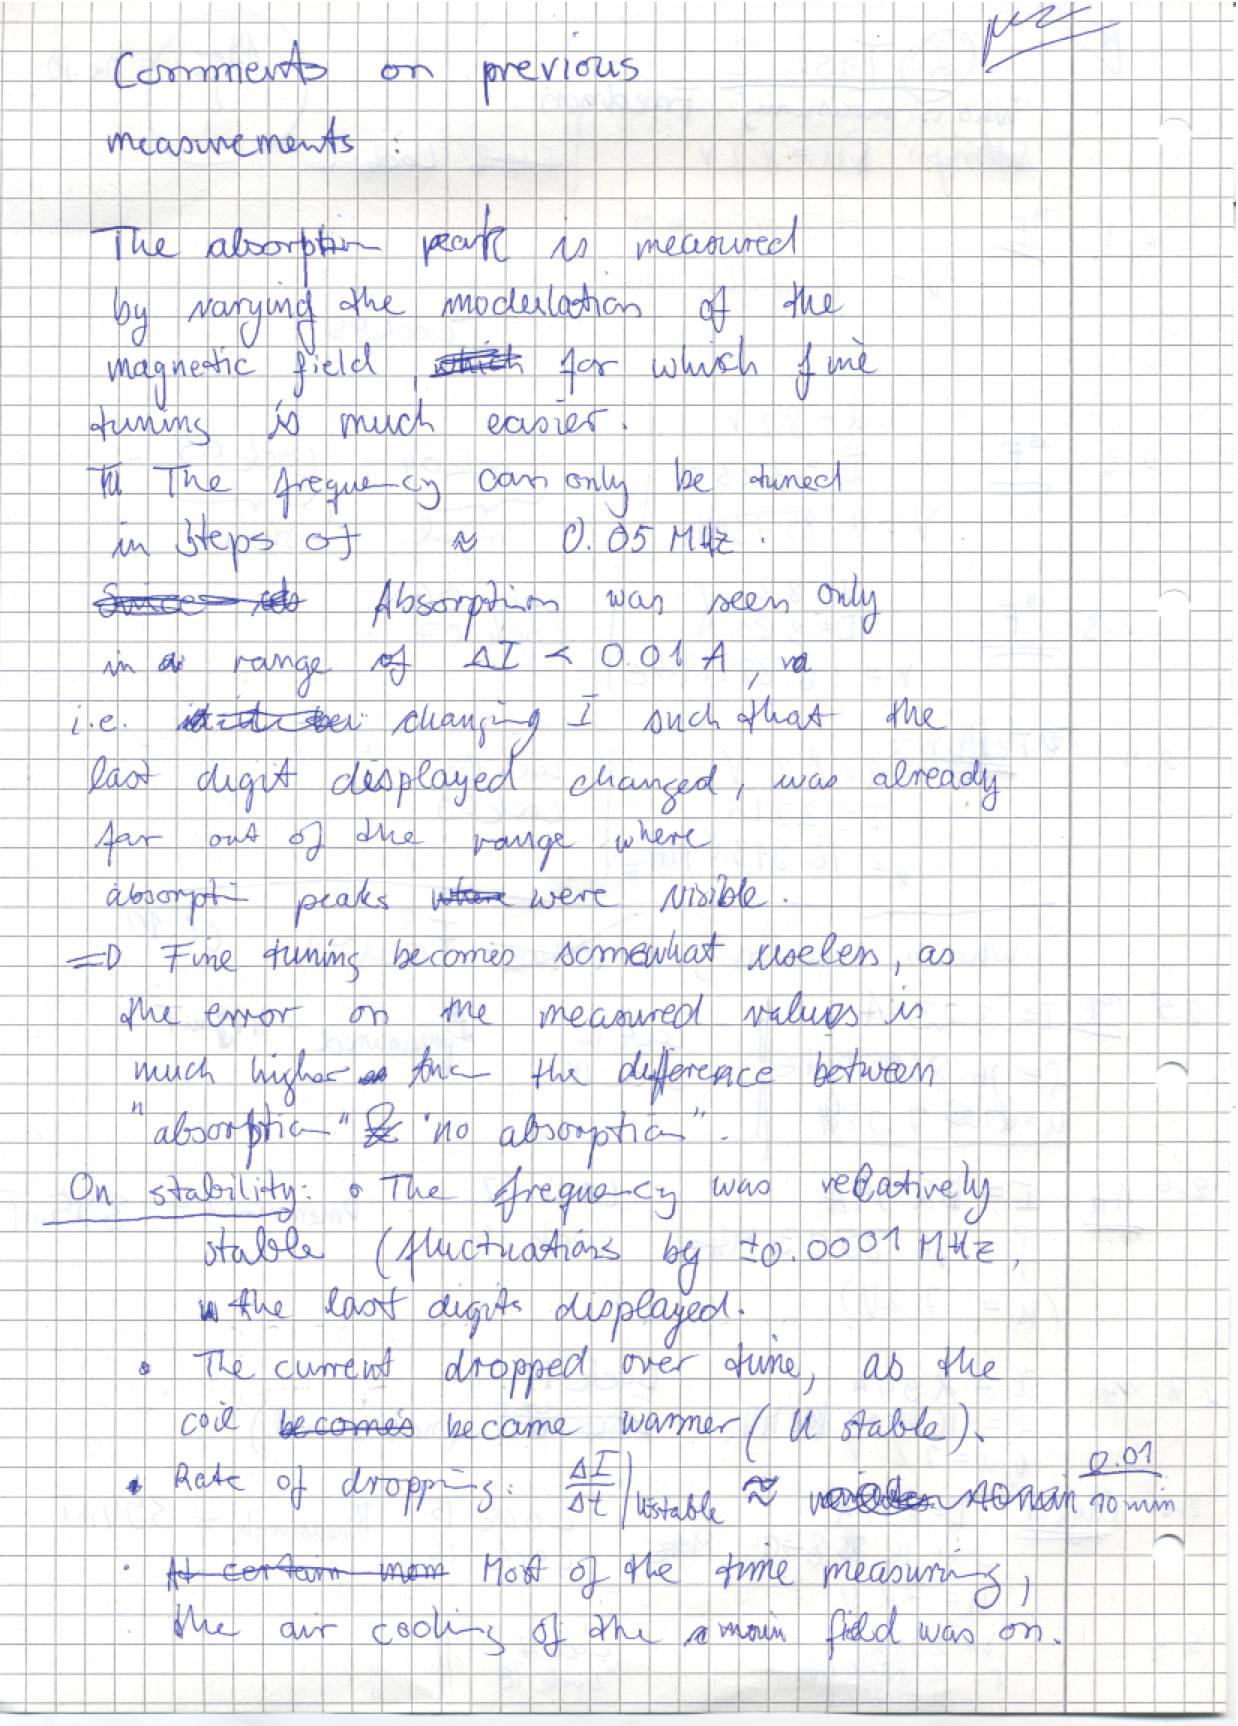
\includegraphics[width=\linewidth]{appendix/spin4.jpg}
\clearpage
    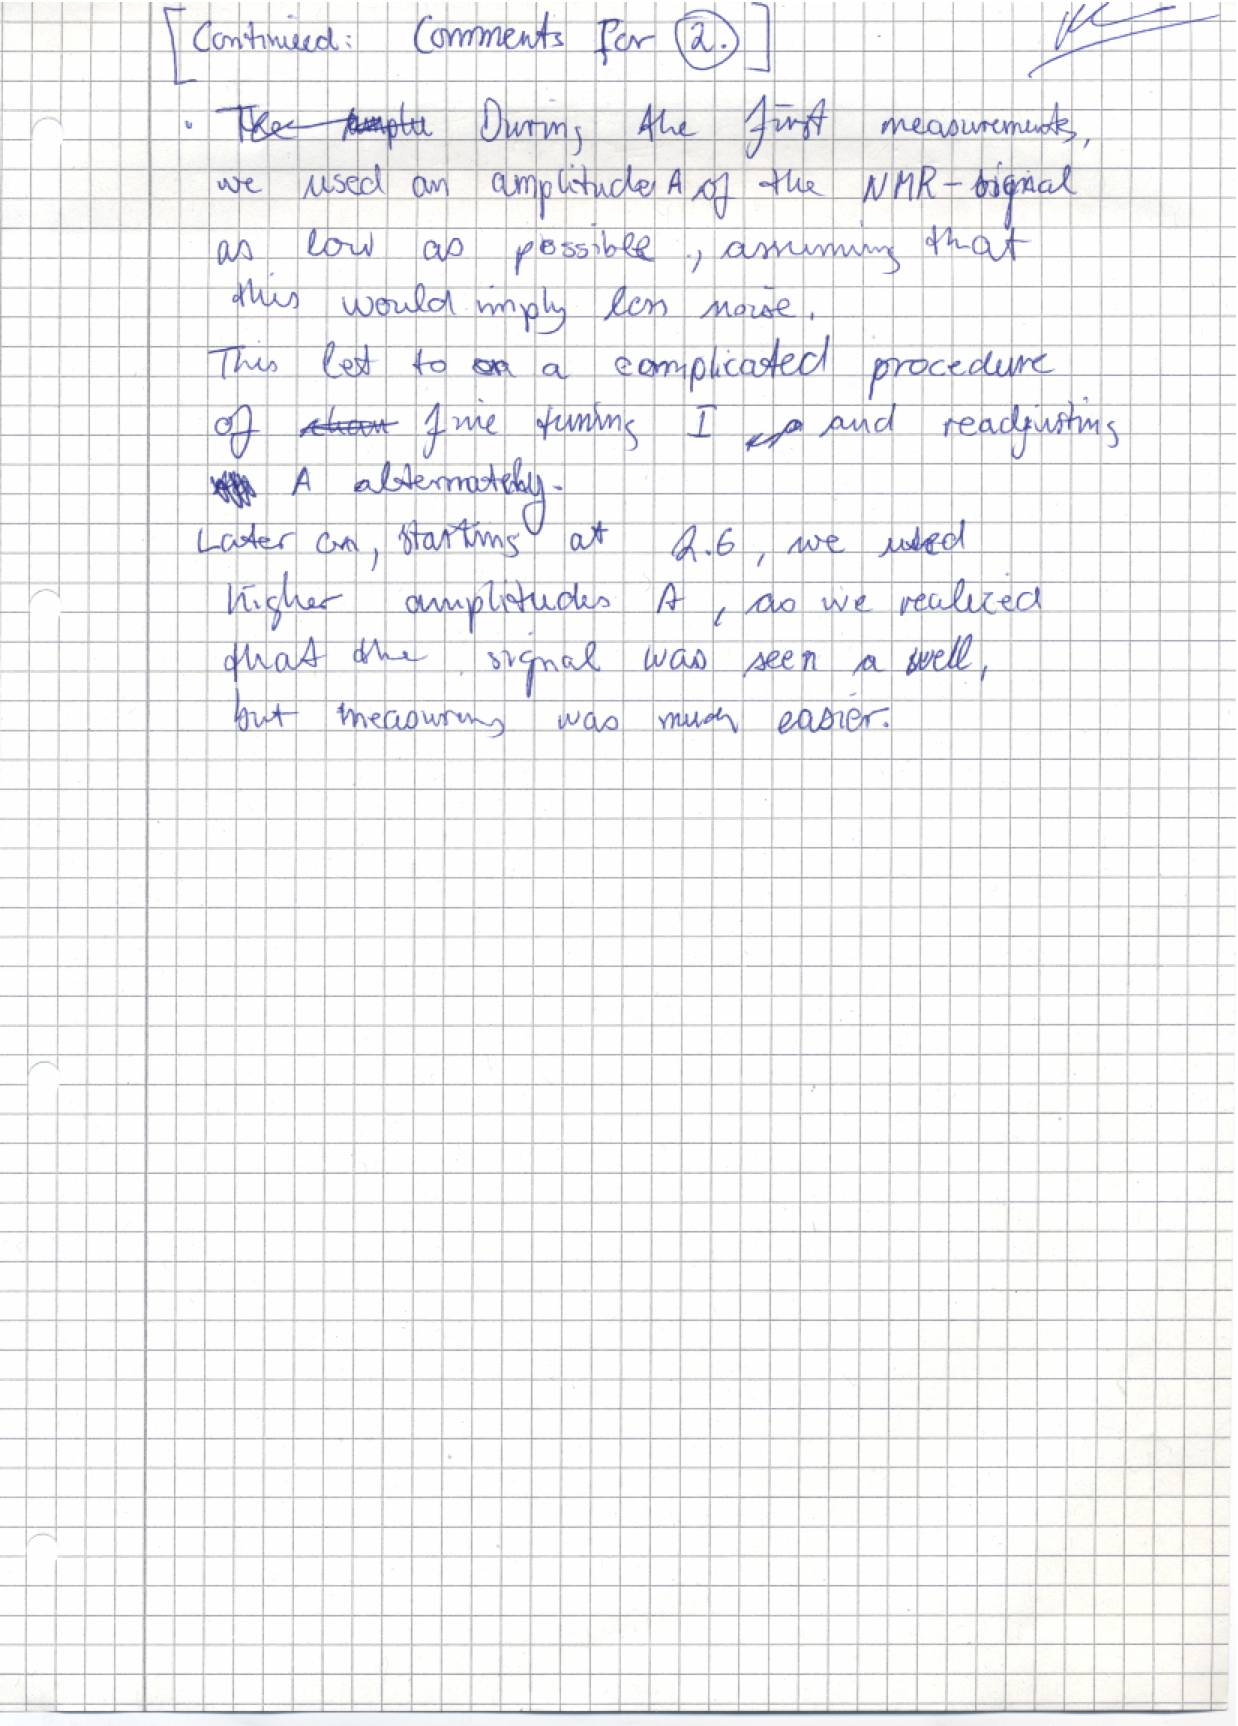
\includegraphics[width=\linewidth]{appendix/spin5.jpg}
\clearpage
    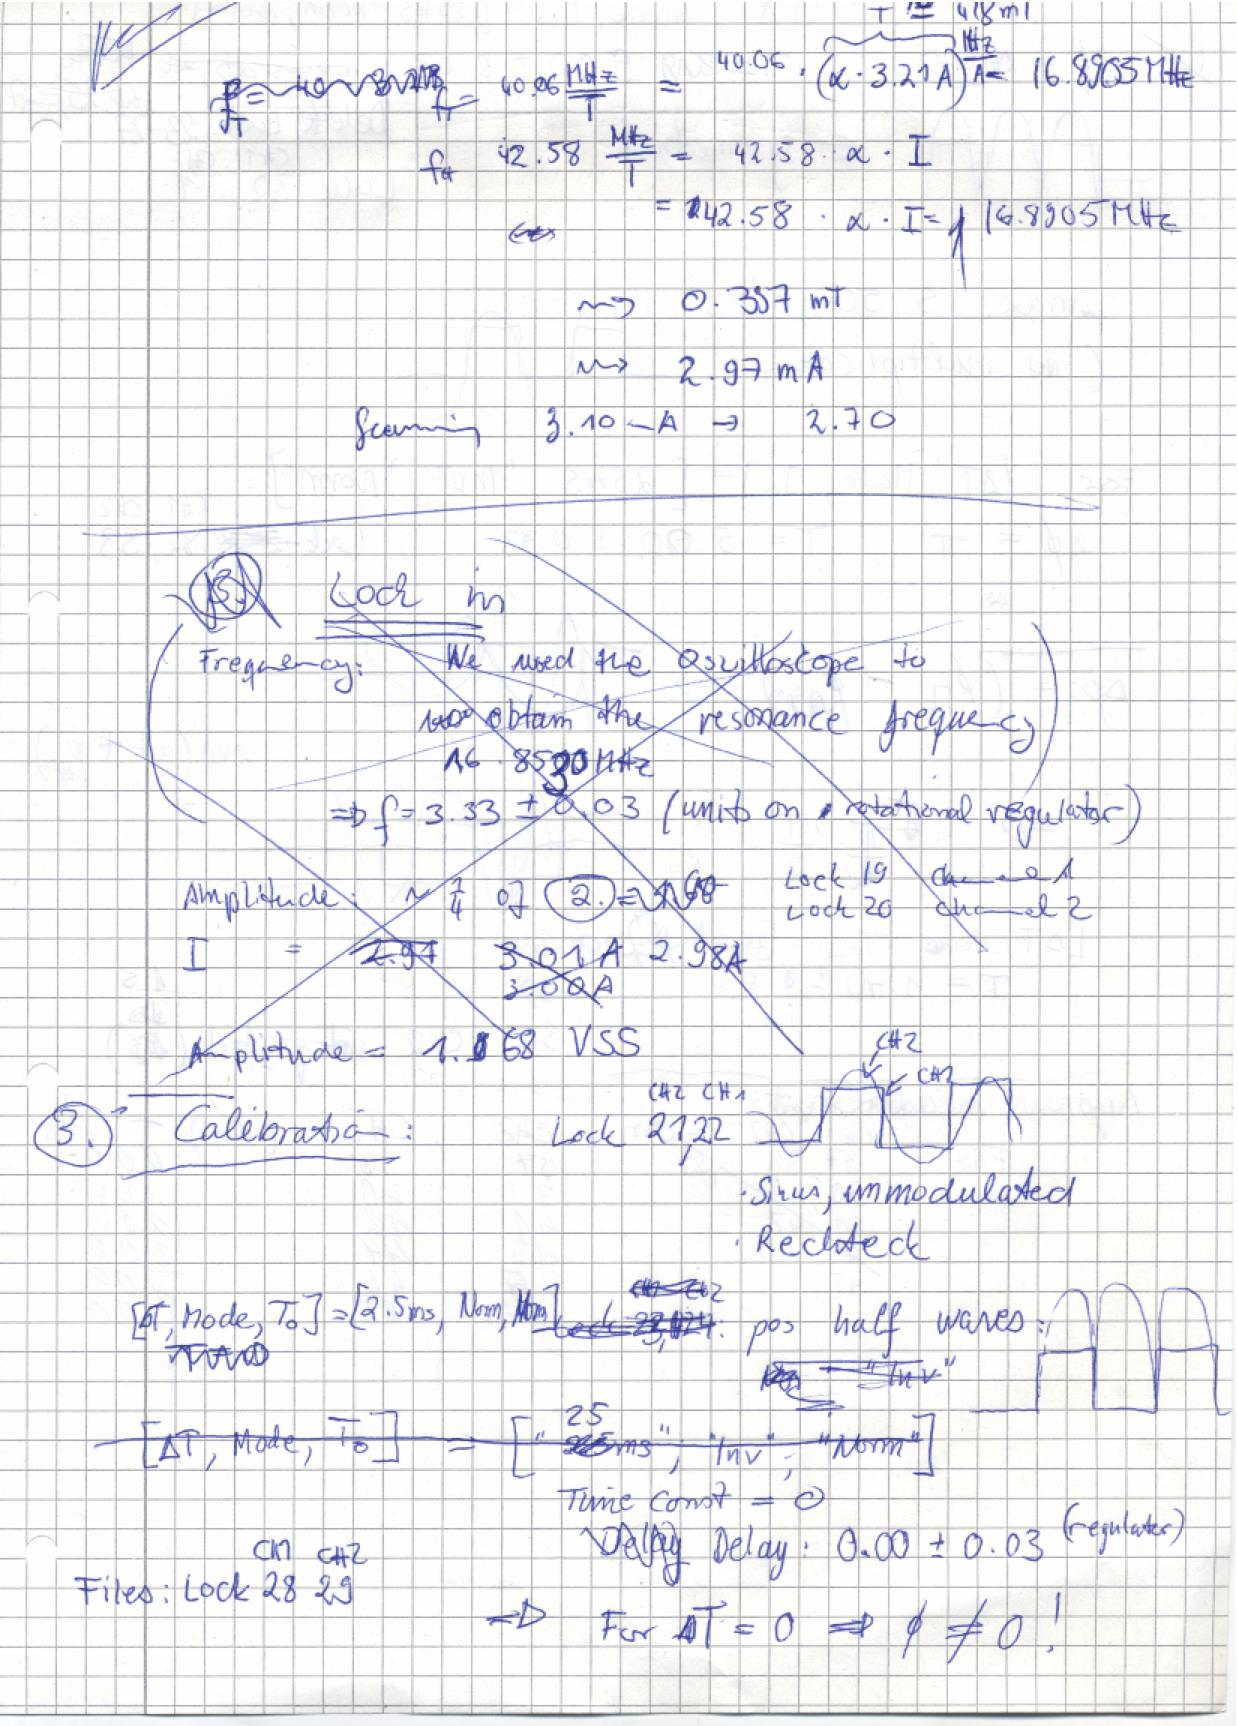
\includegraphics[width=\linewidth]{appendix/spin6.jpg}
\clearpage
    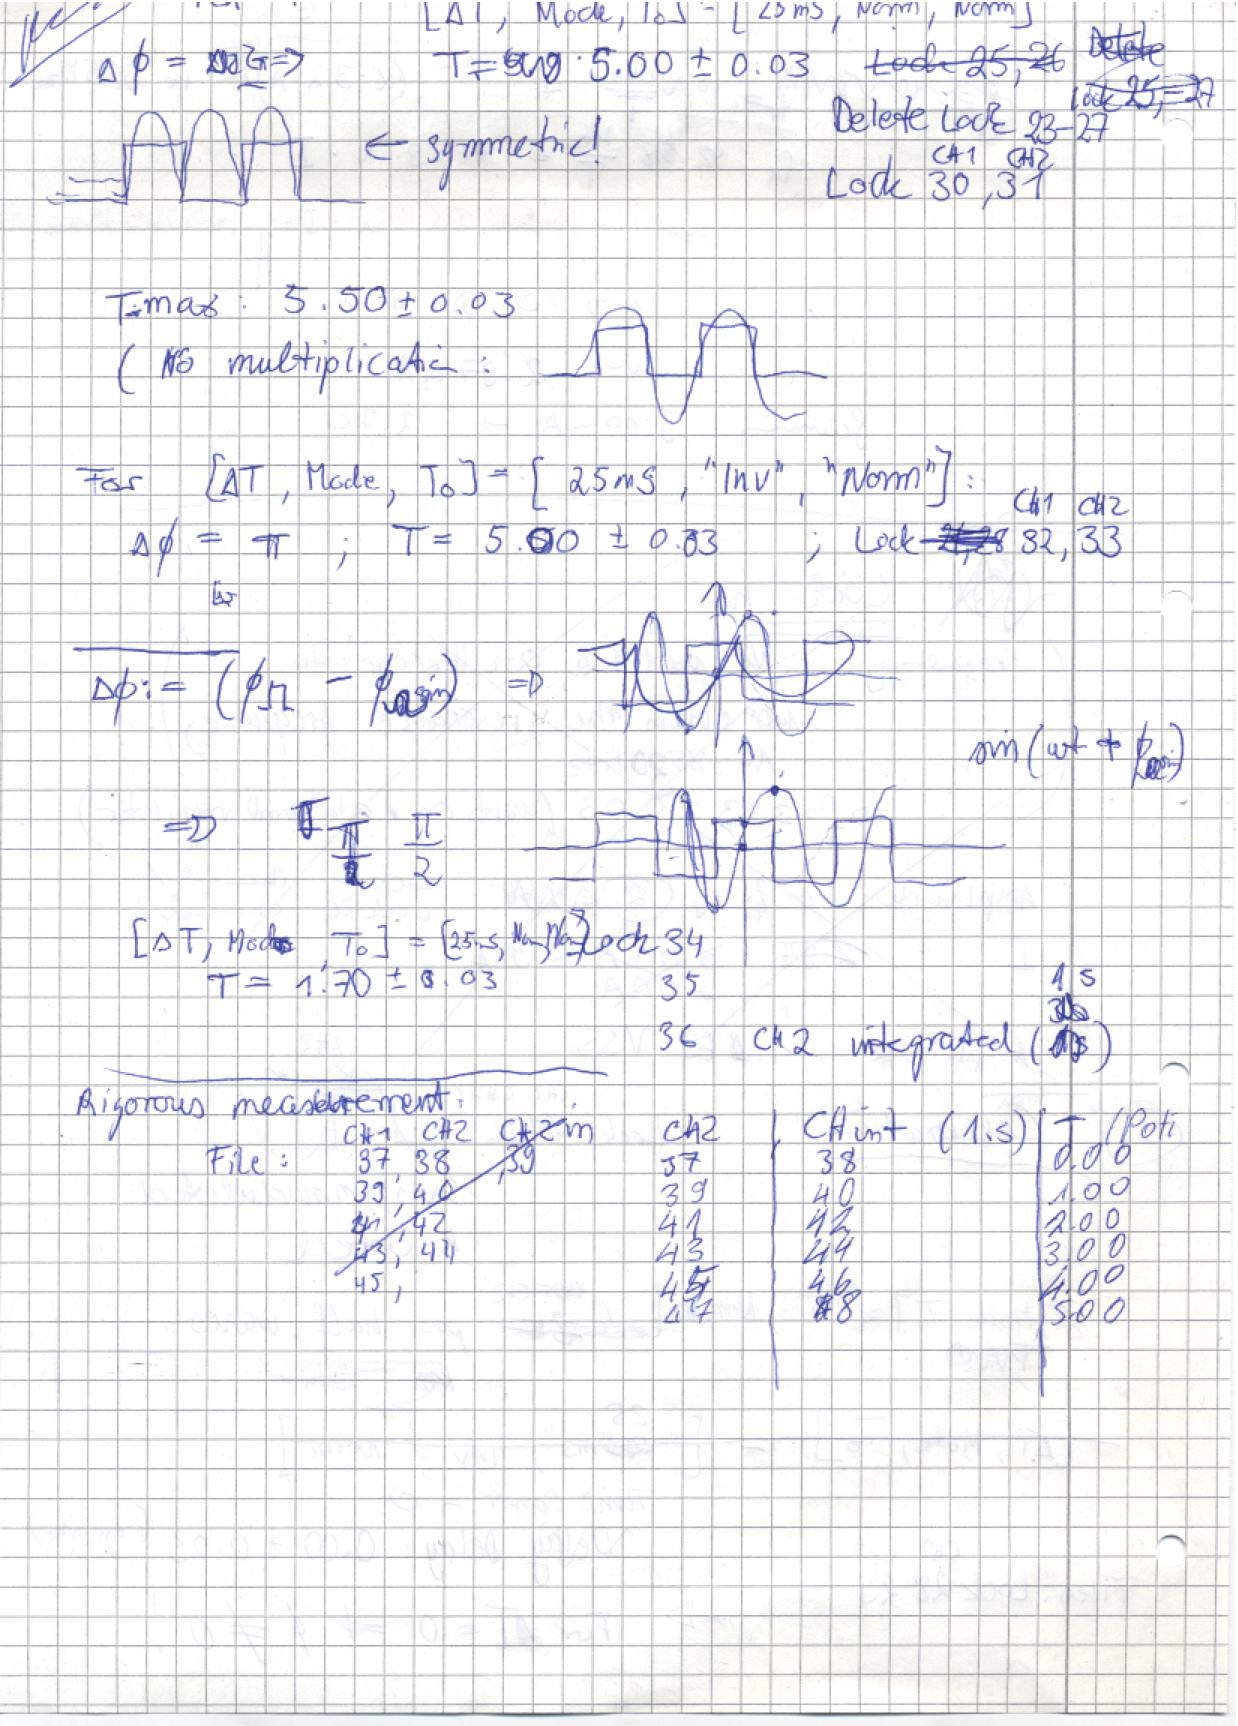
\includegraphics[width=\linewidth]{appendix/spin7.jpg}
\clearpage



\end{document}
